%%%%%%%%%%%%%%%%%%%%%%%%%%%%%%%%%%%%%%%%%%%%%%%%%%%%%%%%%%%%%%%%%%%%%%%%%%%%%%%%
% Template for USENIX papers.
%
% History:
%
% - TEMPLATE for Usenix papers, specifically to meet requirements of
%   USENIX '05. originally a template for producing IEEE-format
%   articles using LaTeX. written by Matthew Ward, CS Department,
%   Worcester Polytechnic Institute. adapted by David Beazley for his
%   excellent SWIG paper in Proceedings, Tcl 96. turned into a
%   smartass generic template by De Clarke, with thanks to both the
%   above pioneers. Use at your own risk. Complaints to /dev/null.
%   Make it two column with no page numbering, default is 10 point.
%
% - Munged by Fred Douglis <douglis@research.att.com> 10/97 to
%   separate the .sty file from the LaTeX source template, so that
%   people can more easily include the .sty file into an existing
%   document. Also changed to more closely follow the style guidelines
%   as represented by the Word sample file.
%
% - Note that since 2010, USENIX does not require endnotes. If you
%   want foot of page notes, don't include the endnotes package in the
%   usepackage command, below.
% - This version uses the latex2e styles, not the very ancient 2.09
%   stuff.
%
% - Updated July 2018: Text block size changed from 6.5" to 7"
%
% - Updated Dec 2018 for ATC'19:
%
%   * Revised text to pass HotCRP's auto-formatting check, with
%     hotcrp.settings.submission_form.body_font_size=10pt, and
%     hotcrp.settings.submission_form.line_height=12pt
%
%   * Switched from \endnote-s to \footnote-s to match Usenix's policy.
%
%   * \section* => \begin{abstract} ... \end{abstract}
%
%   * Make template self-contained in terms of bibtex entires, to allow
%     this file to be compiled. (And changing refs style to 'plain'.)
%
%   * Make template self-contained in terms of figures, to
%     allow this file to be compiled. 
%
%   * Added packages for hyperref, embedding fonts, and improving
%     appearance.
%   
%   * Removed outdated text.
%
%%%%%%%%%%%%%%%%%%%%%%%%%%%%%%%%%%%%%%%%%%%%%%%%%%%%%%%%%%%%%%%%%%%%%%%%%%%%%%%%

\documentclass[letterpaper,twocolumn,10pt]{article}
\usepackage{usenix-2020-09}

% to be able to draw some self-contained figs
\usepackage{tikz}
\usepackage{amsmath}

% customize packages
\usepackage{listings}
\usepackage{titlesec}
\titleformat{\paragraph}
{\normalfont\normalsize\bfseries}{\theparagraph}{1em}{}
\titlespacing*{\paragraph}
{0pt}{3.25ex plus 1ex minus .2ex}{1.5ex plus .2ex}

% inlined bib file
% \usepackage{natbib}
% \usepackage{biblatex}

\lstset{
  aboveskip=3mm,
  belowskip=3mm,
  showstringspaces=false,
  columns=flexible,
  basicstyle={\small\ttfamily},
  numbers=none,
  numberstyle=\tiny\color{gray},
  keywordstyle=\color{blue},
  commentstyle=\color{dkgreen},
  stringstyle=\color{mauve},
  breaklines=true,
  breakatwhitespace=true,
  tabsize=3
}

%-------------------------------------------------------------------------------
\begin{document}
%-------------------------------------------------------------------------------

%don't want date printed
\date{\today}

% make title bold and 14 pt font (Latex default is non-bold, 16 pt)
\title{\Large \bf CSE221:\\
  Operating System Benchmark}

%for single author (just remove % characters)
\author{
{\rm Alex Martakis}\\
University of California, San Diego
\and
{\rm Johnathan Huynh}\\
University of California, San Diego
\and
{\rm Xinhao Luo}\\
University of California, San Diego
% copy the following lines to add more authors
% \and
% {\rm Name}\\
%Name Institution
} % end author

\maketitle


% Keep things handy: if you need to look up some styles, check backup.tex!

%-------------------------------------------------------------------------------
\section{Introduction}
%-------------------------------------------------------------------------------

In this report, our goal is to gain further understanding of a complex system, more specifically an operating system that is commonly used today. Our goal is to learn to experiment, benchmark, and test the performance of a system in order to gain an understanding of its characteristics.

To ensure the methodology of the experiment is thorough, each member was responsible for contributing to each procedure by running their own tests and code in order to obtain repeatable and consistent results. With this approach, it is ensured that each member is aware of every concept and able to provide insight into each step of the process. We believe this approach minimizes pitfalls and leads to a methodical and in-depth analysis of the subject at hand.

For our experiments, we utilized C as our language of choice and GCC as our preferred compiler with option -O0 and gcc (GCC) 10.3.0. With this system we do not expect to run into any significant implications on this environment. We estimate this project will take approximately 50 hours to complete. After completing the project, we believe we originally underestimated the time and spent over 80 hours on the project.
% @TODO by Tuesday

%-------------------------------------------------------------------------------
\section{Machine Description}
%-------------------------------------------------------------------------------

We have come up with a custom machine branded in SuperMicro, with X9DRI-LN4F+ motherboard, built with the following specs: 
\begin{description}
  
\item[Processor] Intel(R) Xeon(R) CPU E5-2670 v2 \footnote{Source from \href{https://www.cpu-world.com/CPUs/Xeon/Intel-Xeon\%20E5-2670\%20v2.html}{cpu-world}} \\ 10 Cores 20 Threads
\item[Cycle Time] 1/2.5Ghz = 0.4ns
\item[L1 cache] 320 KiB 8-way set associative instruction caches; 320 KiB 8-way set associative data caches
\item[L2 cache] 2.5 MiB 8-way set associative caches
\item[L3 cache] 25 MiB 20-way set associative shared cache
\item [Instruction] 64 bit
\item[Memory bus] DDR3; Clock 1333Mhz, Width 64 bits 
\item[I/O bus] PCIe Express and SATA\footnote{The BIOS is modded to use NVMe as the Boot device}
\item[RAM size] 40192M, 40G
\item[Disk] Sabrent Rocket NVMe PCIe M.2 2280 SSD 256G
\item[Disk Speed] up to 3100 MB/s (read) and 1050 MB/s (write)\footnote{\href{https://www.sabrent.com/product/SB-ROCKET-256/256gb-rocket-nvme-pcie-m-2-2280-internal-ssd-high-performance-solid-state-drive/\#description}{Merchandise Introduction}}
\item[Network card] on board RJ45 network card
\item[Speed] 1Gbit/s
\item[Operating System] Linux NixOS 5.10.57 \\ 21.11pre130979.gfedcba (Porcupine)
\end{description}

\noindent

Note that machine has two CPU so the cache size is actually double. However, we have disabled one CPU and set CPU affinity to a single core when running the test. 

Also, we locked the CPU to 2Ghz since its frequency will only be stable under that setting, even with turbo turned off. The machine we used is from recycle center, and it is expected some of its specs is not stable. 

%-------------------------------------------------------------------------------
\section{Operations}
%-------------------------------------------------------------------------------
\subsection{CPU, Scheduling, and OS Services}

\subsubsection{Measurement overhead}

%In this section, we will report the overhead of reading time, and report the overhead of using a loop to measure many iterations of an operation.

\paragraph{Methodology}

This portion's main goal is first to benchmark the overhead of reading the clock, and second to measure the overhead of loops. \\
\textit{Overhead of reading time}\\
Inspired by \cite{paoloni2010benchmark}, we will use the RDTSCP function supported by our Intel CPU in order to read the time-stamp counter. By reading the time-stamp counter twice and recording the average difference between the two readings we can get the overhead of RDTSCP which will be the overhead of reading the clock. The difference between the two time-stamps after reading the clock twice will be the time that the system takes to read the clock. \\
 \textit{Overhead of using a loop}\\
To benchmark the overhead of using a loop we will create a loop with no statements. The counter for this loop will also be initialized outside of the declaration of the loop in order to not factor in that time either. This inner loop will be a simple loop structure with nothing in the loop. We will check the time of the clock before the start of the loop and after the end of the loop. This loop will run a certain constant number of times, and then the difference in time will be divided by the amount of times the loop ran in order to calculate the overhead of the loop.

\paragraph{Estimate}
\textit{Overhead of reading time}\\
According to what we have found from other users testing with RDTSCP (\href{https://community.intel.com/t5/Software-Tuning-Performance/High-impact-of-rdtsc/td-p/1092539}{Intel Forum RDTSCP Discussion}), it is said that RDTSCP will roughly take around 30 cycles. With a singular cycle time from our machine description being 0.4 ns we get the overhead prediction to be $30$ cycles $\times \frac{0.4 ns}{1\ cycle} = 12 ns$. We will use RDTSCP to read the clock and by reading the clock twice and taking the difference we will be able to get the overhead of reading time.
 \\
  \textit{Overhead of using a loop} \\
 Over a large sample we will get the average loop overhead. Looking at the assembly code for an empty for loop (examined through \href{https://godbolt.org/z/Por6xoP41}{godbolt}) we see a loop without any content takes about 5 cycles to operate. With this we estimate the overhead of a loop is $5 cycles \times \frac{0.4 ns}{1\ cycle} = 1.25 ns$.

\paragraph{Results}

Results presented are CPU cycles. Each measurement is a trial of 1000 iterations.

\begin{enumerate}
    \item [Reading Time]
        \begin{center}
            \begin{tabular}{||c c||} 
             \hline
             Measurements & Avg \\ [0.5ex] 
             \hline\hline
             1 & 64.708  \\ 
             \hline
             2 & 64.503  \\ 
             \hline
             3 & 63.285  \\ 
             \hline
             4 & 64.739 \\ 
             \hline
             5 & 65.576  \\ 
             \hline
             \hline
            \end{tabular} \\
            \begin{tabular}{||c c||} 
             \hline
             Total Avg & Std-dev \\ [0.5ex] 
             \hline\hline
             64.562 & 0.737 \\ 
             \hline
             \hline
            \end{tabular}
        \end{center}
    \item [Loop Overhead]
        \begin{center}
            \begin{tabular}{||c c||} 
                 \hline
                 Measurements & Avg \\ [0.5ex] 
                 \hline\hline
                 1 & 7.156  \\ 
                 \hline
                 2 & 7.502  \\ 
                 \hline
                 3 & 6.978  \\ 
                 \hline
                 4 & 6.948 \\ 
                 \hline
                 5 & 6.889  \\ 
                 \hline
                 \hline
            \end{tabular} \\
            \begin{tabular}{||c c||} 
                 \hline
                 Total Avg & Std-dev \\ [0.5ex] 
                 \hline\hline
                 7.095 & 0.222 \\ 
                 \hline
                \hline
            \end{tabular}
        \end{center}
\end{enumerate}

\paragraph{Analysis}

 \textit{Overhead of reading time}\\
 The overhead of the clock was over twice the amount of cycles as predicted. Our prediction was lower than the actual overhead of reading the clock, we believe there may be more factors to causing increased overhead that we did not incorporate to our prediction such as speed of the I/O bus, instructions taking more cycles than usual, these special instructions to read the clock taking a longer time to get results. The standard deviation is low enough to support the accuracy of our final average for reading the clock. Our prediction for the cycle count of loop overhead was similar to that of the result. Loop overhead incurs on average a little more than two cycles over what we predicted. We speculate our prediction is lower because some instructions for the loop take longer than a single clock cycle such as the jmp instruction. The standard deviation for our experiment is quite low enough supporting the accuracy of our results for loop overhead.

\subsubsection{Procedure call overhead}

%Report as a function of number of integer arguments from 0-7. What is the increment overhead of an argument?

\paragraph{Methodology}

In order to gauge the procedure call overhead, we tested ten different functions that all had a different number of arguments. The parameter sizes varied from 0 to 10. An example of something that might attribute to significant delay would be that the program will need to access some location in the memory before it can begin. We will be testing the difference in time stamps between the values over 1000 times. After this, the average values will be computed. % @TODO by Tuesday

\paragraph{Estimate}

$ O = Overhead \\ $
$ n = parameters \\$
$ T = time \\$
$ C = Clock Cycle \\$

We expect:

$T = C * n + O \\$
\hspace{.1cm}
Therefore, as the number of parameters increase for a given function, the estimate that the product of clock cycles and \emph{n parameters} will increase the overall Time when taking into account the constant overhead.

\paragraph{Results}
Results are in CPU cycles.
\begin{enumerate}
    \item [Process]
        \begin{center}
            \begin{tabular}{||c c||} 
             \hline
             Zero Parameter & Avg \\ [0.5ex] 
             \hline\hline
             1 & 58.56  \\ 
             \hline
             2 & 57.531  \\ 
             \hline
             3 & 59.764  \\ 
             \hline
             4 & 108.204 \\ 
             \hline
             5 & 73.2286  \\ 
             \hline
             \hline
            \end{tabular}
                            \begin{tabular}{||c c||} 
                 \hline
                 Total Avg & Std-dev \\ [0.5ex] 
                 \hline\hline
                 73.229 & 19.720\\ 
                 \hline
                \hline
            \end{tabular}
        \end{center}
        \item [Process]
        \begin{center}
            \begin{tabular}{||c c||} 
             \hline
             One Parameter & Avg \\ [0.5ex] 
             \hline\hline
             1 & 57.903  \\ 
             \hline
             2 & 58.466  \\ 
             \hline
             3 & 59.159  \\ 
             \hline
             4 & 56.974 \\ 
             \hline
             5 & 58.02  \\ 
             \hline
             \hline
            \end{tabular}
            \begin{tabular}{||c c||} 
                 \hline
                 Total Avg & Std-dev \\ [0.5ex] 
                 \hline\hline
                 58.1044 & 0.716\\ 
                 \hline
                \hline
            \end{tabular}
        \end{center}\textbf{}
        \item [Process]
        \begin{center}
            \begin{tabular}{||c c||} 
             \hline
             Two Parameter & Avg \\ [0.5ex] 
             \hline\hline
             1 & 57.813  \\ 
             \hline
             2 & 58.99  \\ 
             \hline
             3 & 59.056  \\ 
             \hline
             4 & 55.422 \\ 
             \hline
             5 & 57.652  \\ 
             \hline
             \hline
            \end{tabular}
                \begin{tabular}{||c c||} 
                 \hline
                 Total Avg & Std-dev \\ [0.5ex] 
                 \hline\hline
                 57.7866 & 1.3167\\ 
                 \hline
            \end{tabular}
        \end{center}
        \item [Process]
        \begin{center}
            \begin{tabular}{||c c||} 
             \hline
             Three Parameter & Avg \\ [0.5ex] 
             \hline\hline
             1 & 57.908  \\ 
             \hline
             2 & 101.066  \\ 
             \hline
             3 & 58.653  \\ 
             \hline
             4 & 59.602 \\ 
             \hline
             5 & 59.328  \\ 
             \hline
             \hline
            \end{tabular}
            \begin{tabular}{||c c||} 
                 \hline
                 Total Avg & Std-dev \\ [0.5ex] 
                 \hline\hline
                 67.3114 & 16.887\\ 
                 \hline
                \hline
            \end{tabular}
        \end{center}
        \item [Process]
        \begin{center}
            \begin{tabular}{||c c||} 
             \hline
             Four Parameter & Avg \\ [0.5ex] 
             \hline\hline
             1 & 59.704  \\ 
             \hline
             2 & 60.271  \\ 
             \hline
             3 & 60.302  \\ 
             \hline
             4 & 61.553 \\ 
             \hline
             5 & 61.231  \\ 
             \hline
             \hline
            \end{tabular}
                                        \begin{tabular}{||c c||} 
                 \hline
                 Total Avg & Std-dev \\ [0.5ex] 
                 \hline\hline
                 60.612 & 0.679\\ 
                 \hline
                \hline
            \end{tabular}
        \end{center}
        \item [Process]
        \begin{center}
            \begin{tabular}{||c c||} 
             \hline
             Five Parameter & Avg \\ [0.5ex] 
             \hline\hline
             1 & 61.741  \\ 
             \hline
             2 & 59.646  \\ 
             \hline
             3 & 62.036  \\ 
             \hline
             4 & 59.121 \\ 
             \hline
             5 & 59.458  \\ 
             \hline
             \hline
            \end{tabular}
                                        \begin{tabular}{||c c||} 
                 \hline
                 Total Avg & Std-dev \\ [0.5ex] 
                 \hline\hline
                 60.4004 & 1.230\\ 
                 \hline
                \hline
            \end{tabular}
        \end{center}
        \item [Process]
        \begin{center}
            \begin{tabular}{||c c||} 
             \hline
             Six Parameter & Avg \\ [0.5ex] 
             \hline\hline
             1 & 61.612  \\ 
             \hline
             2 & 60.395  \\ 
             \hline
             3 & 89.038  \\ 
             \hline
             4 & 63.766 \\ 
             \hline
             5 & 64.017  \\ 
             \hline
             \hline
            \end{tabular}
                                        \begin{tabular}{||c c||} 
                 \hline
                 Total Avg & Std-dev \\ [0.5ex] 
                 \hline\hline
                 67.765 & 10.721\\ 
                 \hline
                \hline
            \end{tabular}
        \end{center}
        \item [Process]
        \begin{center}
            \begin{tabular}{||c c||} 
             \hline
             Seven Parameter & Avg \\ [0.5ex] 
             \hline\hline
             1 & 71.347  \\ 
             \hline
             2 & 70.32 \\ 
             \hline
             3 & 68.444  \\ 
             \hline
             4 & 69.19 \\ 
             \hline
             5 & 67.597  \\ 
             \hline
             \hline
            \end{tabular}
                            \begin{tabular}{||c c||} 
                 \hline
                 Total Avg & Std-dev \\ [0.5ex] 
                 \hline\hline
                 69.379 & 1.329\\ 
                 \hline
                \hline
            \end{tabular}
        \end{center}
\end{enumerate}

\paragraph{Analysis}

When analysing the gathered results, we can see that our original estimate is correct. The average time it took for each process to execute, increased as the number of parameters increased. The difference between the smallest and largest parameter, differed anywhere from 10 to 20 nanoseconds. This makes sense due to the additional processing that must occur. However, it should be noted that there were outliers such as the 4th test for the Zero Parameter. This odd time could be a result of a larger than average overhead for that process. The system may have been prioritizing another process a higher priority than the method for that test.

\subsubsection{System call overhead}

%Report the cost of a minimal system call. How does it compare to the cost of a procedure call? Note that some operating systems will cache the results of some system calls (e.g., idempotent system calls like getpid), so only the first call by a process will actually trap into the OS.

\paragraph{Methodology}

While NixOS has properties that are different to Linux OS, such as the way it is distributed, NixOS uses the same Linux kernel. Therefore, operations such as system calls, will have similar executions methods. In this section, our goal is to report the cost of a minimal system call and then compare it to the cost of the procedure call. Here, we utilized the benchmark 'getpid' as the system call. 'getpid' is a good bench mark because it mitigates the system call overhead. As seen in $3.1.2$ a function with no parameters is what mitigates the overhead. This call will be executed 1000 times and then the mean and standard deviation will be acquired.

\paragraph{Estimate}

Due to this call being from an application and not from the system itself, we estimate that this system call will be much greater in comparison to the procedure call.% @TODO by Tuesday

\paragraph{Results}

\begin{enumerate}
    \item [Process]
        \begin{center}
            \begin{tabular}{||c c||} 
             \hline
             System Call & Avg \\ [0.5ex] 
             \hline\hline
             1 & 12324.07  \\ 
             \hline
             2 & 12444.35  \\ 
             \hline
             3 & 12296.075  \\ 
             \hline
             4 & 12482.37 \\ 
             \hline
             5 & 12345.125  \\ 
             \hline
             \hline
            \end{tabular}
            \begin{tabular}{||c c||} 
                 \hline
                 Total Avg & Std-dev \\ [0.5ex] 
                 \hline\hline
                 12378.398 & 72.104\\ 
                 \hline
                \hline
            \end{tabular}
        \end{center}
\end{enumerate}

\paragraph{Analysis}

When analysing the data from the test, we can see that our original estimate was correct. The average time of the system call overhead is significantly higher than the procedure call's avg time. When assessing why this is the case, these larger times can be due to attributes in this method involving the application and not just the system itself. The system call procedure can be seen taking as much as two-hundred times longer to process when compared to the procedure call procedure.

\subsubsection{Task creation time}

%Report the time to create and run both a process and a kernel thread (kernel threads run at user-level, but they are created and managed by the OS; e.g., pthread_create on modern Linux will create a kernel-managed thread). How do they compare?

\paragraph{Methodology}

In order to create new processes, we may use fork(). To limit other possible interferences, each fork will do nothing and exit immediately after creation, and the parent process will just start counting and waiting for the exit. It is also noticeable that since this creation process may be pretty short and exiting and return may also have extra overhead, we repeat this process for 1000 times and calculate the average cpu cycles. RDTSC() will be used during the measurement.

Similarly for kernel threads, we may use pthread\_create() instead of fork(), and pthread\_join() instead of wait(); then do the calculation.

\paragraph{Estimate}

Overhead may include a if statement control flow where it helps to identify parents and child. However, we won't do heavy operations after it. Mis-predict and inhibit branching won't be part of the consideration. Without these side effects, cost of the if statement itself is cheap and can be ignored. RDTSC() will be fetched once and based on the previous analysis, it is also a pretty small factor. 

It is pretty hard to find any reference for this hardware directly, so we would take a relative value based on other's benchmark result, which mimic our single core situation \footnote{\href{https://stackoverflow.com/questions/52175375/overhead-in-creating-a-thread-vs-process-on-linux}{benchmark with python}}. It is expected that the thread creation cycles will way less than process creation cycles. Also, even though fork is doing COW (copy-on-write), other operations e.g. assigning new process id, environment inheritance, etc.. may still take some time. It is believed to be a pretty expensive operation while thread creation will be better.

\paragraph{Results}

The results here are CPU cycles

\begin{enumerate}
    \item [Process]
        \begin{center}
            \begin{tabular}{||c c||} 
                 \hline
                 Iterations & Avg \\ [0.5ex] 
                 \hline\hline
                 1 & 585008.545 \\ 
                 \hline
                 2 & 584898.235  \\ 
                 \hline
                 3 & 585801.865 \\ 
                 \hline
                 4 & 586973.265 \\ 
                 \hline
                 5 & 586067.395  \\ 
                 \hline
                 \hline
            \end{tabular} 
            \begin{tabular}{||c c||} 
                 \hline
                 Total Avg & Std-dev \\ [0.5ex] 
                 \hline\hline
                 585749.861 & 758.296 \\ 
                 \hline
                \hline
            \end{tabular}
        \end{center}
    \item [Thread]
        \begin{center}
            \begin{tabular}{||c c||} 
                 \hline
                 Iterations & Avg \\ [0.5ex] 
                 \hline\hline
                 1 & 169652.575 \\ 
                 \hline
                 2 & 169658.905  \\ 
                 \hline
                 3 & 170016.67 \\ 
                 \hline
                 4 & 168637.26 \\ 
                 \hline
                 5 & 169113.975  \\ 
                 \hline
                 \hline
            \end{tabular} 
            \begin{tabular}{||c c||} 
                 \hline
                 Total Avg & Std-dev \\ [0.5ex] 
                 \hline\hline
                 169415.877 & 484.444 \\ 
                 \hline
                \hline
            \end{tabular}
        \end{center}
\end{enumerate}

\paragraph{Analysis}

The test result matched with the fact that thread creation actually costs a lot less than the process creation and the deviation is pretty small, which means the result is quite stable between iterations, but at the same time the difference is not as high as expected. The possible overhead occurring may be the memory operation when collecting the timestamp, so we actually count more than than we need. Using pipe to pass the timestamp, or collecting the timestamp in the parent thread (assuming the memory operation is less than function overhead) will be a better choice.

\subsubsection{Context switch time}

%Report the time to context switch from one process to another, and from one kernel thread to another. How do they compare? In the past students have found using blocking pipes to be useful for forcing context switches.

\paragraph{Methodology}

To measure the context switch time, we need to have two processes working together, so we have a parent process and fork a new process, and before switching to the new process, we record the count cycles. Then we use a block pipe to read from child to ensure our child has switched to. We can then compare the count and time. However, we need to make sure that our machine is running in single core mode. RDTSC() will be used during the measurement. 

\paragraph{Estimate}

Still, there is an overhead of if statement to identify parent/child and assign local variables for RDTSC() counts. 

There are some benchmark out there stating average being $5 \mu s$ \footnote{\href{https://docs.microsoft.com/en-us/gaming/gdk/_content/gc/system/overviews/finding-threading-issues/high-context-switches}{Microsoft Report}}. We may compare this result by dividing our cycle times by the frequency. Also, context switches may experience lots of steps e.g. saving registrars. It is expected to be a relatively expensive operation.

\paragraph{Results}

The results here are CPU cycles

\begin{enumerate}
    \item [Process]
        \begin{center}
            \begin{tabular}{||c c||} 
             \hline
             Iterations & Avg \\ [0.5ex] 
             \hline\hline
             1 & 334230.325  \\ 
             \hline
             2 & 332975.165  \\ 
             \hline
             3 & 333658.920  \\ 
             \hline
             4 & 333610.660 \\ 
             \hline
             5 & 333622.525  \\ 
             \hline
             \hline
            \end{tabular}
            \begin{tabular}{||c c||} 
             \hline
             Total Avg & Std-dev \\ [0.5ex] 
             \hline\hline
             333619.519 & 397.471 \\ 
             \hline
             \hline
            \end{tabular}
        \end{center}
    \item [Thread]
        \begin{center}
            \begin{tabular}{||c c||} 
                 \hline
                 Iterations & Avg \\ [0.5ex] 
                 \hline\hline
                 1 & 78460.935  \\ 
                 \hline
                 2 & 78360.260  \\ 
                 \hline
                 3 & 79402.530  \\ 
                 \hline
                 4 & 78874.270 \\ 
                 \hline
                 5 & 79037.530 \\ 
                 \hline
                 \hline
            \end{tabular} \\
            \begin{tabular}{||c c||} 
                 \hline
                 Total Avg & Std-dev \\ [0.5ex] 
                 \hline\hline
                 78827.105 & 382.005\\ 
                 \hline
                \hline
            \end{tabular}
        \end{center}
\end{enumerate}

\paragraph{Analysis}

The average trend aligned with the creation process, as switching to a process will have more work to migrate than the thread, which is most likely within the same contexts. However, since we also use mmap when collecting the timestamp, the differences is still a bit smaller than expected, and more than what Microsoft's reported average is as well.

%-------------------------------------------------------------------------------
\subsection{Memory}
%-------------------------------------------------------------------------------

\subsubsection{RAM Access Time}

% Report latency for individual integer accesses to main memory and the L1 and L2 caches. Present results as a graph with the x-axis as the log of the size of the memory region accessed, and the y-axis as the average latency. Note that the lmbench paper is a good reference for this experiment. In terms of the lmbench paper, measure the "back-to-back-load" latency and report your results in a graph similar to Fig. 1 in the paper. You should not need to use information about the machine or the size of the L1, L2, etc., caches when implementing the experiment; the experiment will reveal these sizes. In your graph, label the places that indicate the different hardware regimes (L1 to L2 transition, etc.).

\paragraph{Methodology}

For this experiment we take inspiration and reference from the Imbench paper \cite{mcvoy1996lmbench}. From the paper we will be focusing on the back-to-back latency since this is commonly referred to by software developers as memory latency. \\
We will create various integer lists with different sizes ranging from $2^{15}$ bytes to $2^{30}$ bytes which is roughly 32 kilobytes to 1 gigabyte. We will traverse through these arrays that are in memory with different stride lengths with many samples. The paper mentions that small stride sizes should be high performing because of high spatial locality and larger stride sizes will have poor performance because of prefetching unused data. We will use our timer (which utilizes RDTSCP) to record the start and end time of a memory access. Large lists are utilized because we want to be able to see the changes in memory access throughout L1, L2, L3 cache and main memory and see the various differences in latency. These experiments will be repeated for many times to calculate the average for different array lengths and stride sizes.

\paragraph{Estimate}
To predict measurements for memory latencies we reference \href{https://www.intel.com/content/dam/www/public/us/en/documents/manuals/64-ia-32-architectures-optimization-manual.pdf}{Intel manual} for the Sandy Bridge microarchitecture and look at the fastest latency recorded for each level of data/cache and we provide more conservative estimates, and we look at \href{http://norvig.com/21-days.html#answers}{this article} for references on memory access times.\\
Hardware prediction:
\begin{itemize}
    \item L1: 4-6 cycles
    \item L2: 12-16 cycles
    \item L3: 44-70 cycles
    \item Main memory DRAM: 120-150 cycles
\end{itemize}
Software prediction:\\
We do not expect there to be very much software overhead in accessing memory as the main portion of this is waiting for the memory to be loaded. This ld instruction to load memory most likely has "zero" latency or very negligible time compared to the actual time to be accessing memory. 
\paragraph{Results}
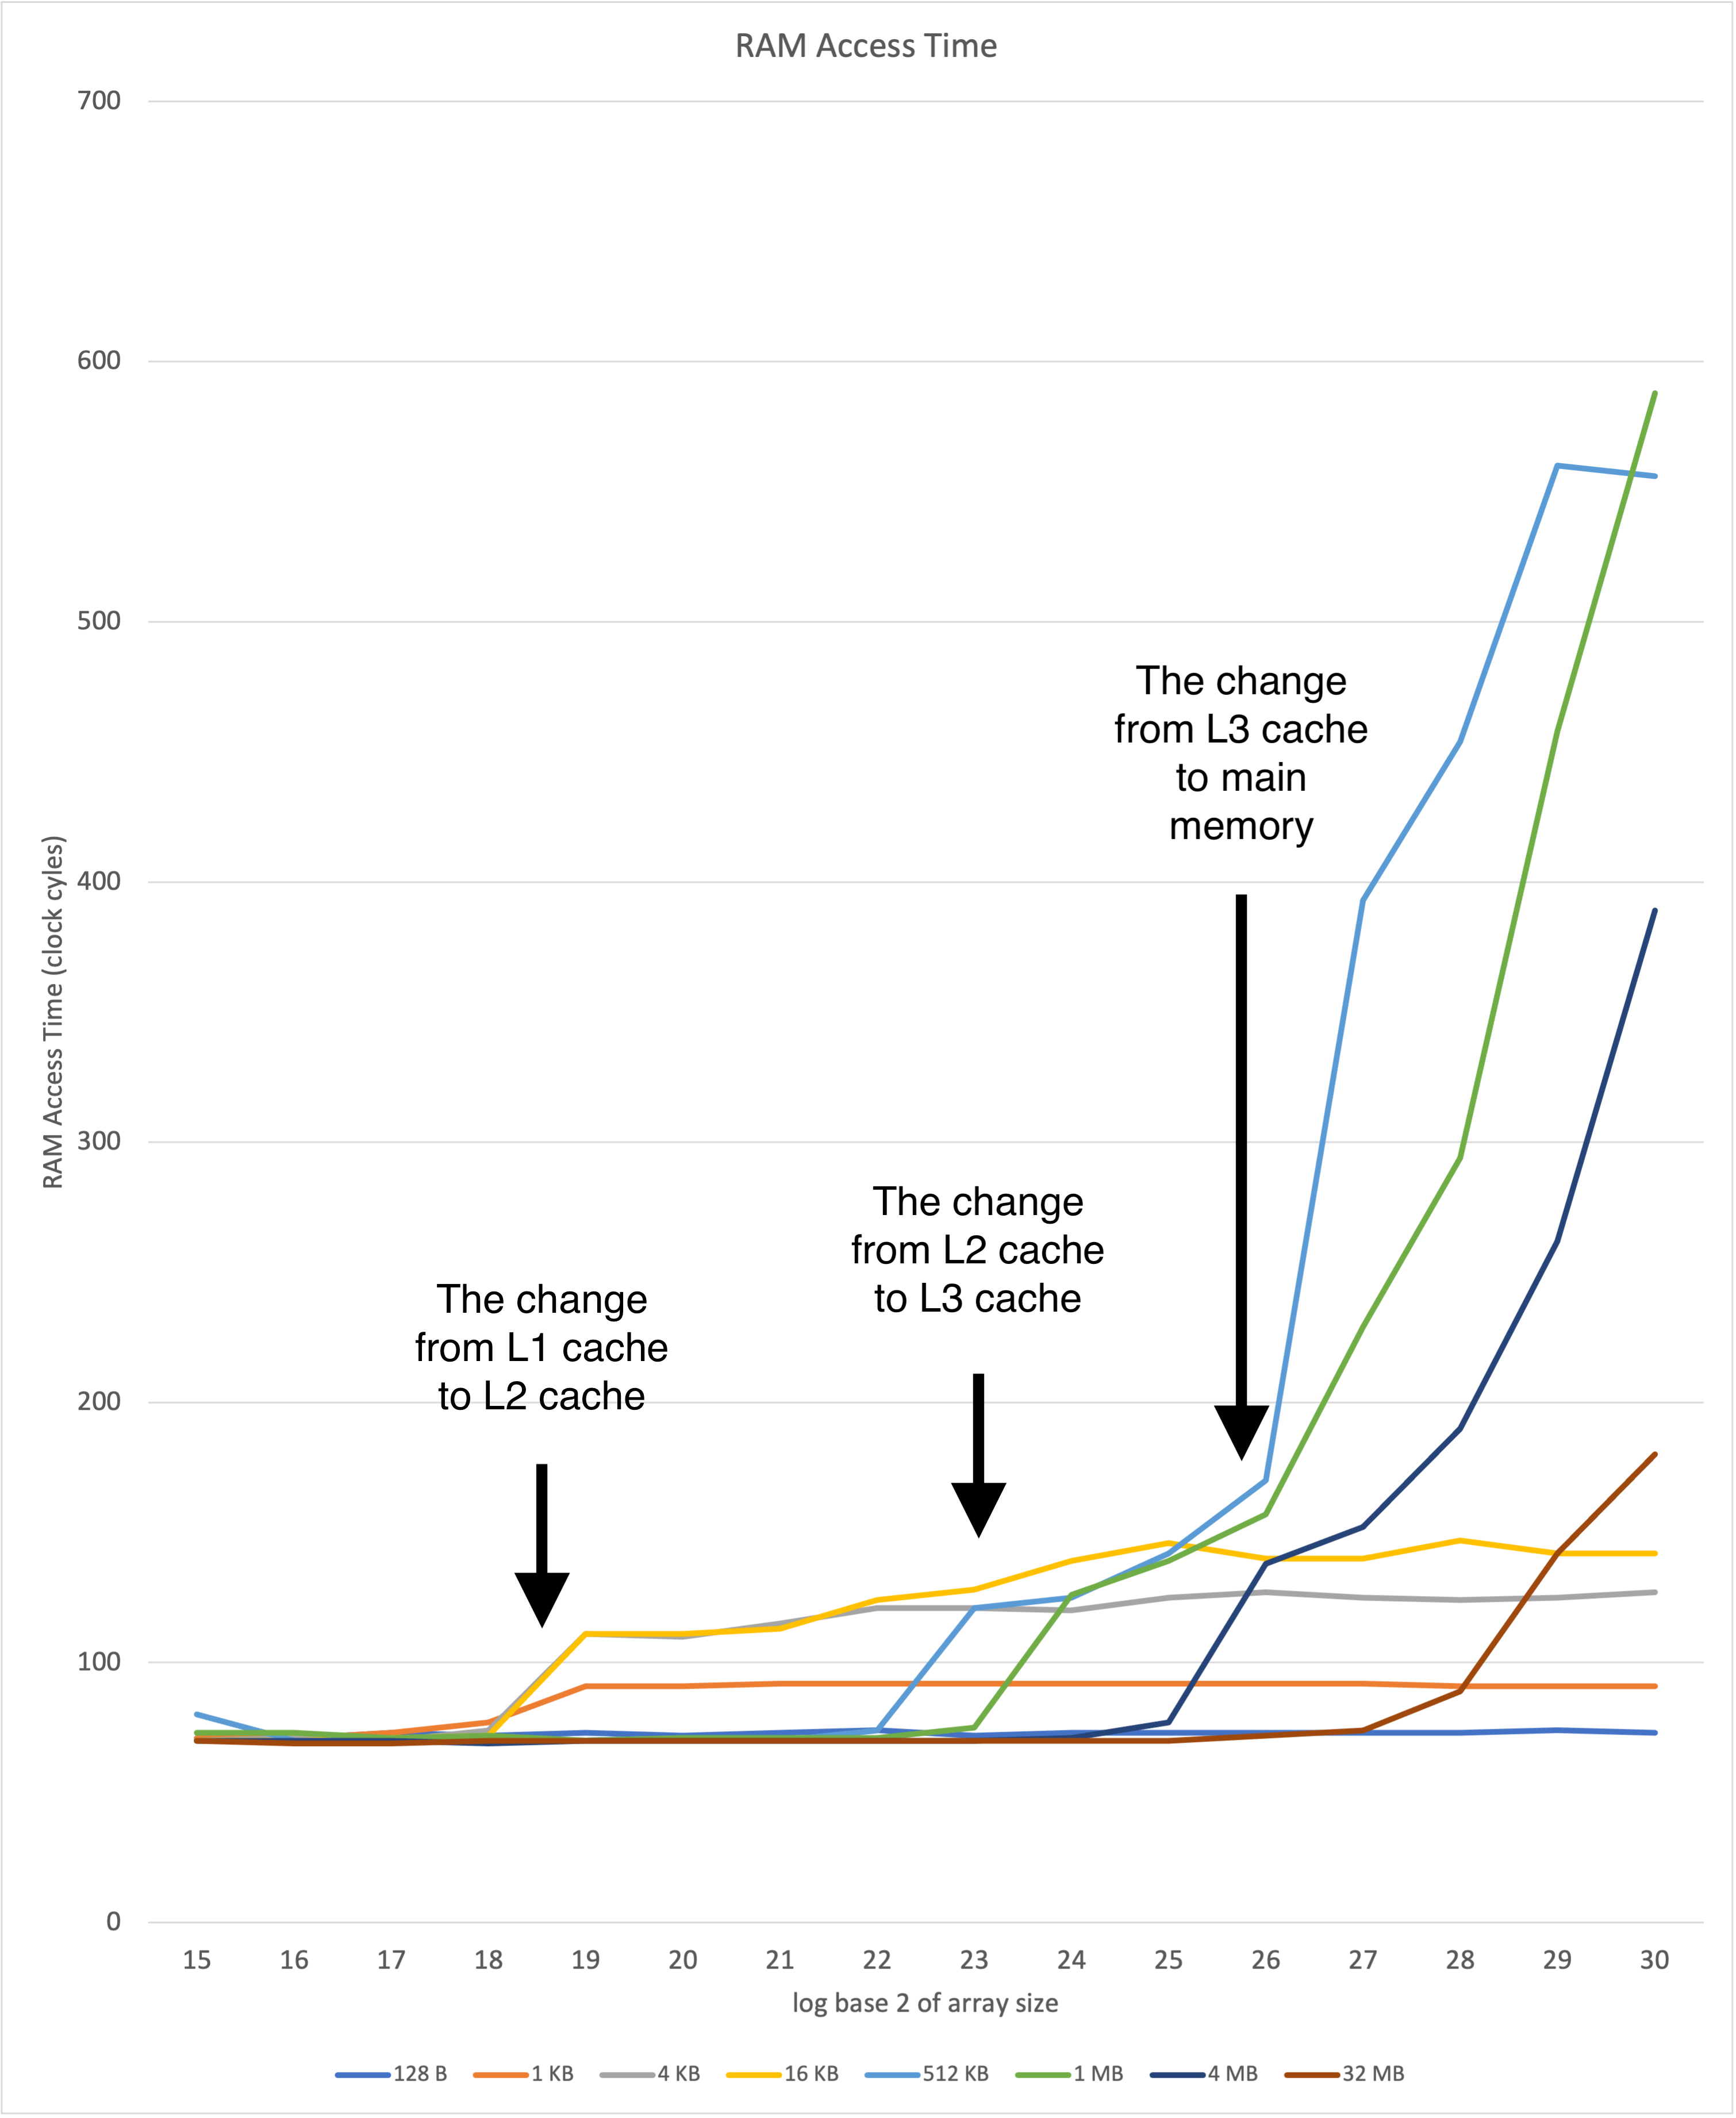
\includegraphics[width=7.5cm]{ram_access_time.png}

\paragraph{Analysis}

The results produced in our graph differ from our predictions by a hefty amount of clock cycles. The amount of clock cycles recorded for a memory access started at around 70 cycles, when we had predicted about 4-6 cycles for L1 cache. The lines on our graph are different from the Imbench paper as we do not have the same plateau shape that was on the paper. Our graph grows more linearly rather than a sudden jolt of increase in cycles for many of our stride lengths. There are some stride lengths that do follow the Imbench paper's pattern though. Such as the 1KB stride plateauing in its access time when it hits around 500KB of array size and onwards. Our results take many more cycles than what we actually predicted and we reason this to be various potential factors such as failing to prefetch data and other overheads.
\\


\subsubsection{RAM bandwidth}
% Report bandwidth for both reading and writing. Use loop unrolling to get more accurate results, and keep in mind the effects of cache line prefetching (e.g., see the lmbench paper).
    
\paragraph{Methodology}

To calculate the bandwidth, we may first do some read/write operations with some number of bytes touched, and measure the time elapsed for these operations:

\begin{equation}
    Bandwidth = \frac{\text{\# of byte read/write}}{\text{total elapsed time}}
\end{equation}


However, it is also possible that these operations 1) hit the write policy 2) affects by the prefetching mechanism. To avoid these effects, we could set a larger trunk so that the cache will be bypassed. Furthermore, loop unrolling was also used for a more accurate result.

\paragraph{Estimate}

We have 2 CPUs but each of them has their own memory lines, so we have single channel memory for each of them \footnote{\href{https://www.intel.com/content/www/us/en/support/articles/000056722/processors/intel-core-processors.html}{Calculation reference}}

\begin{equation}
    1333Mhz * 64 / 8 * 1 \approx 10000 MB/s
\end{equation}

\paragraph{Results}

The results here are MB/s

\begin{enumerate}
    \item [Read]
        \begin{center}
            \begin{tabular}{||c c||} 
             \hline
             Iterations & Avg \\ [0.5ex] 
             \hline\hline
             1 & 6946.111  \\ 
             \hline
             2 & 7941.494  \\ 
             \hline
             3 & 7874.829  \\ 
             \hline
             4 & 7843.296 \\ 
             \hline
             5 & 7856.500  \\ 
             \hline
             \hline
            \end{tabular} \\
            \begin{tabular}{||c c||} 
             \hline
             Total Avg & Std-dev \\ [0.5ex] 
             \hline\hline
             7692.446 & 374.692 \\ 
             \hline
             \hline
            \end{tabular}
        \end{center}
    \item [Write]
        \begin{center}
            \begin{tabular}{||c c||} 
                 \hline
                 Iterations & Avg \\ [0.5ex] 
                 \hline\hline
                 1 & 8423.493  \\ 
                 \hline
                 2 & 8219.271  \\ 
                 \hline
                 3 & 8408.419  \\ 
                 \hline
                 4 & 8529.340 \\ 
                 \hline
                 5 & 8409.711   \\ 
                 \hline
                 \hline
                \end{tabular} \\
                \begin{tabular}{||c c||} 
                 \hline
                 Total Avg & Std-dev \\ [0.5ex] 
                 \hline\hline
                 8398.047 & 100.089 \\ 
                 \hline
                \hline
            \end{tabular}
        \end{center}
\end{enumerate}

\paragraph{Analysis}

The result is actually pretty close to a single memory performance. However, the write back in our test seems to be affected by the write back cache. We have tried to invalidate it by obfuscating the memory with memcpy, but write back mode still relieves part of our "abnormal" behavior, which might be the cause of the difference. It is also worth mentioning that our memory are ECC memory, which may incur extra cost compared to normal one.

It is also worth mentioning that the standard derivation is small which means the result is stable. There are still rooms for optimization but at this point our direction is correct.


\subsubsection{Page fault service time} 

%Report the time for faulting an entire page from disk (mmap is one useful mechanism). Dividing by the size of a page, how does it compare to the latency of accessing a byte from main memory?

\paragraph{Methodology}

Page faults can be used to dramatically improve Linux's performance. Ideally, you want the OS to have as few page faults as possible. When a process improperly accesses a memory page, the CPU's memory management unit raises an exception, signaling that a page fault has occurred. More specifically, because of Linux's use of virtual memory for contiguous benefits, a page fault is when a process is mapped to the virtual memory address space but the physical memory has yet to load the process.

For this experiment, utilizing the 'mmap' command. Using this method, will allow us access to a multitude of features with the memory. We first have the method read lines from an image to fill up the ram. We then use the 'mmap' function within our process to play with the memory and create page faults.

\paragraph{Estimate}

We currently estimate that the more demanding the process is, the higher the number of pgouts/s there will be and thus, a higher number of page faults. We currently estimate that the latency between the main memory and the paging will be significant difference when comparing the time.  

\paragraph{Results}

\begin{enumerate}
    \item [Page Fault]
        \begin{center}
            \begin{tabular}{||c c||} 
             \hline
             Iterations & Avg \\ [0.5ex] 
             \hline\hline
             1 & 6.8  \\ 
             \hline
             2 & 6.9  \\ 
             \hline
             3 & 7.0  \\ 
             \hline
             4 & 6.8 \\ 
             \hline
             5 & 6.7  \\ 
             \hline
             \hline
            \end{tabular} \\

                \begin{tabular}{||c c||} 
                 \hline
                 Total Avg & Std-dev \\ [0.5ex] 
                 \hline\hline
                 6.8 & 0.102\\ 
                 \hline
                \hline
            \end{tabular}
            \end{center}
        \end{enumerate}

\paragraph{Analysis}

When running our program we found the average Page Fault Service Time was 6.8 microseconds on average. We defined our page size to be 4096KB. This gives us 4,194,304 bytes. 6800 can be divided by this number of bytes to convert to nanoseconds. Therefore, the estimated time per byte would be 0.0016 nanoseconds per byte.
%-------------------------------------------------------------------------------
\subsection{Network}
%-------------------------------------------------------------------------------

%Evaluate for the TCP protocol. For each quantity, compare both remote and loopback interfaces. Comparing the remote and loopback results, what can you deduce about baseline network performance and the overhead of OS software? For both round trip time and bandwidth, how close to ideal hardware performance do you achieve? In describing your methodology for the remote case, either provide a machine description for the second machine (as above), or use two identical machines.

\paragraph{Environment Setup}

\begin{itemize}
    \item Network Setup: \\ In our network setup, we have a MikroTik CRS354-48G-4S+2Q+RM as our network switch between two machines. Both machines are set up with a IPv6 Address. It is worth mentioning that compared with IPv4, IPv6 may incur more overheads. 
    \item Remote Machine: \\
        We have come up with a Dell R720, built with the following specs: 
        
        \begin{description}
          
        \item[Processor] Intel(R) Xeon(R) CPU E5-2690 v2 \footnote{Source from \href{https://www.cpu-world.com/CPUs/Xeon/Intel-Xeon\%20E5-2690\%20v2.html}{cpu-world}} \\ 10 Cores 20 Threads
        \item[Cycle Time] 1/3Ghz = 0.333ns
        \item[L1 cache] 320 KiB 8-way set associative instruction caches; 320 KiB 8-way set associative data caches
        \item[L2 cache] 2.5 MiB 8-way set associative caches
        \item[L3 cache] 25 MiB 20-way set associative shared cache
        \item [Instruction] 64 bit
        \item[Memory bus] DDR3; Clock 1833Mhz, Width 64 bits 
        \item[I/O bus] PCIe Express and SATA
        \item[RAM size] 128G
        \item[Disk] Kingston NV1 NVMe PCIe M.2 2280 SSD 1T
        \item[Disk Speed] up to 2100 MB/s (read) and 1700 MB/s (write)\footnote{\href{https://www.kingston.com/unitedstates/en/ssd/nv1-nvme-pcie-ssd}{Merchandise Introduction}}
        \item[Network card] Dell onboard fiber channel
        \item[Speed] 10Gbit/s
        \item[Operating System] Linux NixOS 5.10.57 \\ 21.11pre130979.gfedcba (Porcupine)
        \end{description}
\end{itemize}

We specifically choose a better specification machine to avoid bottleneck from the remote side, and both switch and the remote machine are connected and run under 10G speed. Switch is using hardware offload.

\subsubsection{Round trip time}

% Compare with the time to perform a ping (ICMP requests are handled at kernel level).

\paragraph{Methodology}

A typical ping package size is data 56 bytes. In our case, since we are using TCP connection to simulate this, we should first open up a connection between the client and server, and from the clients we send a 56 bytes data. When the server received the data, it should include the exact payload from the request. We could measure the time using between sending the data and fully receiving the response. Also, we may switch the target to localhost when measuring the lo interface, setting up both server and client program locally. We perform the test 100 times for each batch and also test ping the same number of times and get the average.

\paragraph{Estimate}

From the data transfer point of view, 96 (56 + IPv6 overhead, which is around 40 bytes) bytes under 1G/s will be around 0.000768 ms. However, we don't know the latency of the hardware interface, and we have two more of them: 1) switch 2) remote machine, we expected it to be ~ 0.1ms. While the lo interface, it is a virtual device and OS will do all the package routing, where no physical hardware will get involved, which means it is pure OS overhead. We have no idea about how much this overhead will cost but expect to be far less than transferring over network.

\paragraph{Results}

The results here are millisecond

\begin{enumerate}
    \item [lo - Self Impl.]
        \begin{center}
            \begin{tabular}{||c c||} 
             \hline
             Iterations & Avg \\ [0.5ex] 
             \hline\hline
             1 & 0.0554565  \\ 
             \hline
             2 & 0.0550756 \\ 
             \hline
             3 & 0.0557865 \\ 
             \hline
             4 & 0.0561438 \\ 
             \hline
             5 & 0.0557753  \\ 
             \hline
             \hline
            \end{tabular} \\
            \begin{tabular}{||c c||} 
             \hline
             Total Avg & Std-dev \\ [0.5ex] 
             \hline\hline
             0.05564754 & 0.000359 \\ 
             \hline
             \hline
            \end{tabular}
        \end{center}
     \item [lo - Ping]
        \begin{center}
            \begin{tabular}{||c c||} 
             \hline
             Iterations & Avg \\ [0.5ex] 
             \hline\hline
             1 & 0.017  \\ 
             \hline
             2 & 0.019  \\ 
             \hline
             3 & 0.019  \\ 
             \hline
             4 & 0.018 \\ 
             \hline
             5 & 0.017  \\ 
             \hline
             \hline
            \end{tabular} \\
            \begin{tabular}{||c c||} 
             \hline
             Total Avg & Std-dev \\ [0.5ex] 
             \hline\hline
             0.018 & 0.000894 \\ 
             \hline
             \hline
            \end{tabular}
        \end{center}
    \item [Remote - Self Impl.]
        \begin{center}
            \begin{tabular}{||c c||} 
                 \hline
                 Iterations & Avg \\ [0.5ex] 
                 \hline\hline
                 1 & 0.1724719  \\ 
                 \hline
                 2 & 0.173733 \\ 
                 \hline
                 3 & 0.1705358  \\ 
                 \hline
                 4 & 0.1725336 \\ 
                 \hline
                 5 & 0.1731361   \\ 
                 \hline
                 \hline
                \end{tabular} \\
                \begin{tabular}{||c c||} 
                 \hline
                 Total Avg & Std-dev \\ [0.5ex] 
                 \hline\hline
                 0.17248208 & 0.0010754 \\ 
                 \hline
                \hline
            \end{tabular}
        \end{center}
    \item [Remote - Ping]
        \begin{center}
            \begin{tabular}{||c c||} 
                 \hline
                 Iterations & Avg \\ [0.5ex] 
                 \hline\hline
                 1 & 0.188  \\ 
                 \hline
                 2 & 0.188  \\ 
                 \hline
                 3 & 0.187  \\ 
                 \hline
                 4 & 0.178 \\ 
                 \hline
                 5 & 0.187   \\ 
                 \hline
                 \hline
                \end{tabular} \\
                \begin{tabular}{||c c||} 
                 \hline
                 Total Avg & Std-dev \\ [0.5ex] 
                 \hline\hline
                 0.1856 & 0.00382 \\ 
                 \hline
                \hline
            \end{tabular}
        \end{center}
\end{enumerate}

\paragraph{Analysis}

The lo interface measurement can be concluded as purely OS overhead and using it over the result of the over the network measurement, we may get the hardware's latency from this result. \\
While the ping result on the local side, our implementation has higher cost, and the reverse is true on the remote side. We suspect this is because on our program, we using TCP protocol and the kernel on the same machine will have more switch on lo interface, which put more burden on the local machine, while the remote one such situation will be relieving. This result is still believed to be trustworthy since the standard deviation is small, which means the result here is stable, and we have close enough results compared with the ping utils.

\subsubsection{Peak bandwidth}

\paragraph{Methodology}

We may still set up the client and server program and transfer 10 blocks of 1M data, and measure the time accordingly. To avoid unnecessary overhead, we may first prepare the data into the memory, and then send it via the network. We run the test for 10 times per round and 100 times per batch and measure the time. 

\paragraph{Estimate}

In theory, 1MB should take exactly 8 ms to be transfer. However, there are network overheads for each packet (~72 bytes for each, MTU 1500 bytes), so we expect the speed to be ~95\% of the theory value, which is around 8.45ms.

For loop back device, as it is purely software overheads, we expect the speed to be as fast as possible. We know at least several times faster than network card as it is not involved.

\paragraph{Results}

The results here are in milliseconds, for 1 megabyte transferred.

\begin{enumerate}
    \item [lo]
        \begin{center}
            \begin{tabular}{||c c||} 
                 \hline
                 Iterations & Avg \\ [0.5ex] 
                 \hline\hline
                 1 & 0.3320182  \\ 
                 \hline
                 2 & 0.3368662  \\ 
                 \hline
                 3 & 0.336721 \\ 
                 \hline
                 4 & 0.3371553 \\ 
                 \hline
                 5 & 0.3368703   \\ 
                 \hline
                 \hline
                \end{tabular} \\
                \begin{tabular}{||c c||} 
                 \hline
                 Total Avg & Std-dev \\ [0.5ex] 
                 \hline\hline
                 0.3359262 & 0.00195 \\ 
                 \hline
                \hline
            \end{tabular}
        \end{center}
    \item [Remote]
         \begin{center}
            \begin{tabular}{||c c||} 
             \hline
             Iterations & Avg \\ [0.5ex] 
             \hline\hline
             1 & 10.1189782  \\ 
             \hline
             2 & 10.1443683  \\ 
             \hline
             3 & 10.1351207  \\ 
             \hline
             4 & 10.129525 \\ 
             \hline
             5 & 10.1375178 \\ 
             \hline
             \hline
            \end{tabular} \\
            \begin{tabular}{||c c||} 
             \hline
             Total Avg & Std-dev \\ [0.5ex] 
             \hline\hline
             10.133102 & 0.00851 \\ 
             \hline
             \hline
            \end{tabular}
        \end{center}
\end{enumerate}

\paragraph{Analysis}

The loopback devices here achieve around 2976.84MB/s speed which is much higher than the remote one, around 98.68MB/s, 85 percent of the expectation. On the remote side, the bandwidth is lower than the expectation. There are several things to consider: 

\begin{itemize}
    \item Remove unnecessary hardware. Currently we have a switch sitting in the middle and due to some technical limitation, we are unable to remove it for now.
    \item Memory copy is still happening at the remote side, which adds overhead while measuring
    \item TCP slow start seems to be factor as well since we are transferring by 1M block each time, we have observed an increasing speed trend as the test proceeds
\end{itemize}

Measure more data transfer e.g. larger trunk, longer measurement period may be done in the future measurement. It is still worth mentioning that our standard deviation amount batches are stable. 

\subsubsection{Connection overhead} 

% Report setup and tear-down.

\paragraph{Methodology}

When connecting via TCP, the OS perform a four-way handshake, and when (normally) terminate the connection, there will be a four-way handshake (two set of two-way handshake), while it is possible the server will combine the FIN-ACK as one which make it a three-way handshake. We may be measure it by:

\begin{enumerate}
    \item set up a timer and start the connect() process, no data needs to be sent. 
    \item we reset the timer and close() the socket, measure the time. We perform such action 100 times per batch and collect the result.
\end{enumerate}

\paragraph{Estimate}

As a three/four-way handshake, we expect it to be around 2 times of the RTT we measure above. For the teardown, since we are closing connection as client, we only need to send FIN packet and have no need to wait, the loopback device should have similar performance as remote one.

\paragraph{Results}

The results here are in milliseconds

\begin{enumerate}
    \item [lo - Setup]
        \begin{center}
            \begin{tabular}{||c c||} 
             \hline
             Iterations & Avg \\ [0.5ex] 
             \hline\hline
             1 & 0.0804218  \\ 
             \hline
             2 & 0.079161  \\ 
             \hline
             3 & 0.0786141  \\ 
             \hline
             4 & 0.0785565 \\ 
             \hline
             5 & 0.0785603  \\ 
             \hline
             \hline
            \end{tabular} \\
            \begin{tabular}{||c c||} 
             \hline
             Total Avg & Std-dev \\ [0.5ex] 
             \hline\hline
             0.07906274 & 0.000716 \\ 
             \hline
             \hline
            \end{tabular}
        \end{center}
     \item [lo - Tear Down]
        \begin{center}
            \begin{tabular}{||c c||} 
             \hline
             Iterations & Avg \\ [0.5ex] 
             \hline\hline
             1 & 0.0355761  \\ 
             \hline
             2 & 0.0349707  \\ 
             \hline
             3 & 0.0348948  \\ 
             \hline
             4 & 0.0349956 \\ 
             \hline
             5 & 0.0357782  \\ 
             \hline
             \hline
            \end{tabular} \\
            \begin{tabular}{||c c||} 
             \hline
             Total Avg & Std-dev \\ [0.5ex] 
             \hline\hline
             0.03524308 & 0.000361 \\ 
             \hline
             \hline
            \end{tabular}
        \end{center}
    \item [Remote - Setup]
        \begin{center}
            \begin{tabular}{||c c||} 
                 \hline
                 Iterations & Avg \\ [0.5ex] 
                 \hline\hline
                 1 & 0.2301134  \\ 
                 \hline
                 2 & 0.23135  \\ 
                 \hline
                 3 & 0.2221884  \\ 
                 \hline
                 4 & 0.2216165 \\ 
                 \hline
                 5 & 0.2265407   \\ 
                 \hline
                 \hline
                \end{tabular} \\
                \begin{tabular}{||c c||} 
                 \hline
                 Total Avg & Std-dev \\ [0.5ex] 
                 \hline\hline
                 0.22508364 & 0.00309 \\ 
                 \hline
                \hline
            \end{tabular}
        \end{center}
    \item [Remote - Tear down]
        \begin{center}
            \begin{tabular}{||c c||} 
                 \hline
                 Iterations & Avg \\ [0.5ex] 
                 \hline\hline
                 1 & 0.0258408  \\ 
                 \hline
                 2 & 0.0255692  \\ 
                 \hline
                 3 & 0.0257582  \\ 
                 \hline
                 4 & 0.0257662 \\ 
                 \hline
                 5 & 0.02595   \\ 
                 \hline
                 \hline
                \end{tabular} \\
                \begin{tabular}{||c c||} 
                 \hline
                 Total Avg & Std-dev \\ [0.5ex] 
                 \hline\hline
                 0.02565858 & 0.000174 \\ 
                 \hline
                \hline
            \end{tabular}
        \end{center}
\end{enumerate}

\paragraph{Analysis}

From our result, we can see that the setup on loopback device is around 1.5 times of RTT, while the teardown is much slower. The remote side have similar results. We believe that this result pretty much matched our estimate, and since the standard deviation is really small, it could be reproduce stably. The final result should be that the setup is 1.5 times RTT and one packet time for the teardown process.

%-------------------------------------------------------------------------------
\subsection{File System}
%-------------------------------------------------------------------------------


\subsubsection{Size of file cache}

% Note that the file cache size is determined by the OS and will be sensitive to other load on the machine; for an application accessing lots of file system data, an OS will use a notable fraction of main memory (GBs) for the file system cache. Report results as a graph whose x-axis is the size of the file being accessed and the y-axis is the average read I/O time. Do not use a system call or utility program to determine this metric except to sanity check.

\paragraph{Methodology}

For this measurement we will try to figure out this system's file cache size. We will read a file and put it into our main memory. To do this we create a 40 GB randomly generated file before running the experiment. We can utilize this singular file to run each separate file size experiment, this can be done by only reading in a smaller portion of the file for that specific experiment. If the size read in is smaller than the file cache, then this file size will fit within the file system cache. We read the file to bring as much data into the file cache as possible, then it is read a second time to determine if it is read from disk which would take much more time than cache in main memory. If the file size we are at exceeds the file cache size we should see a large increase in read time so when we can see this large change it should it should tell us that the file size is exceeding the file cache size. 

\paragraph{Estimate}

The machine being tested on has 40GB of RAM. Since unused memory that is available can be utilized for the file cache we will predict our file cache size to be the maximum of this 40GB and subtract its current normal memory usage. Using a few commands we can see that our available free memory is about 38-39GB that is not used for any other processes. We predict our file cache size to be somewhere within that range since unused memory can potentially be allocated for the file system cache.

\paragraph{Results}

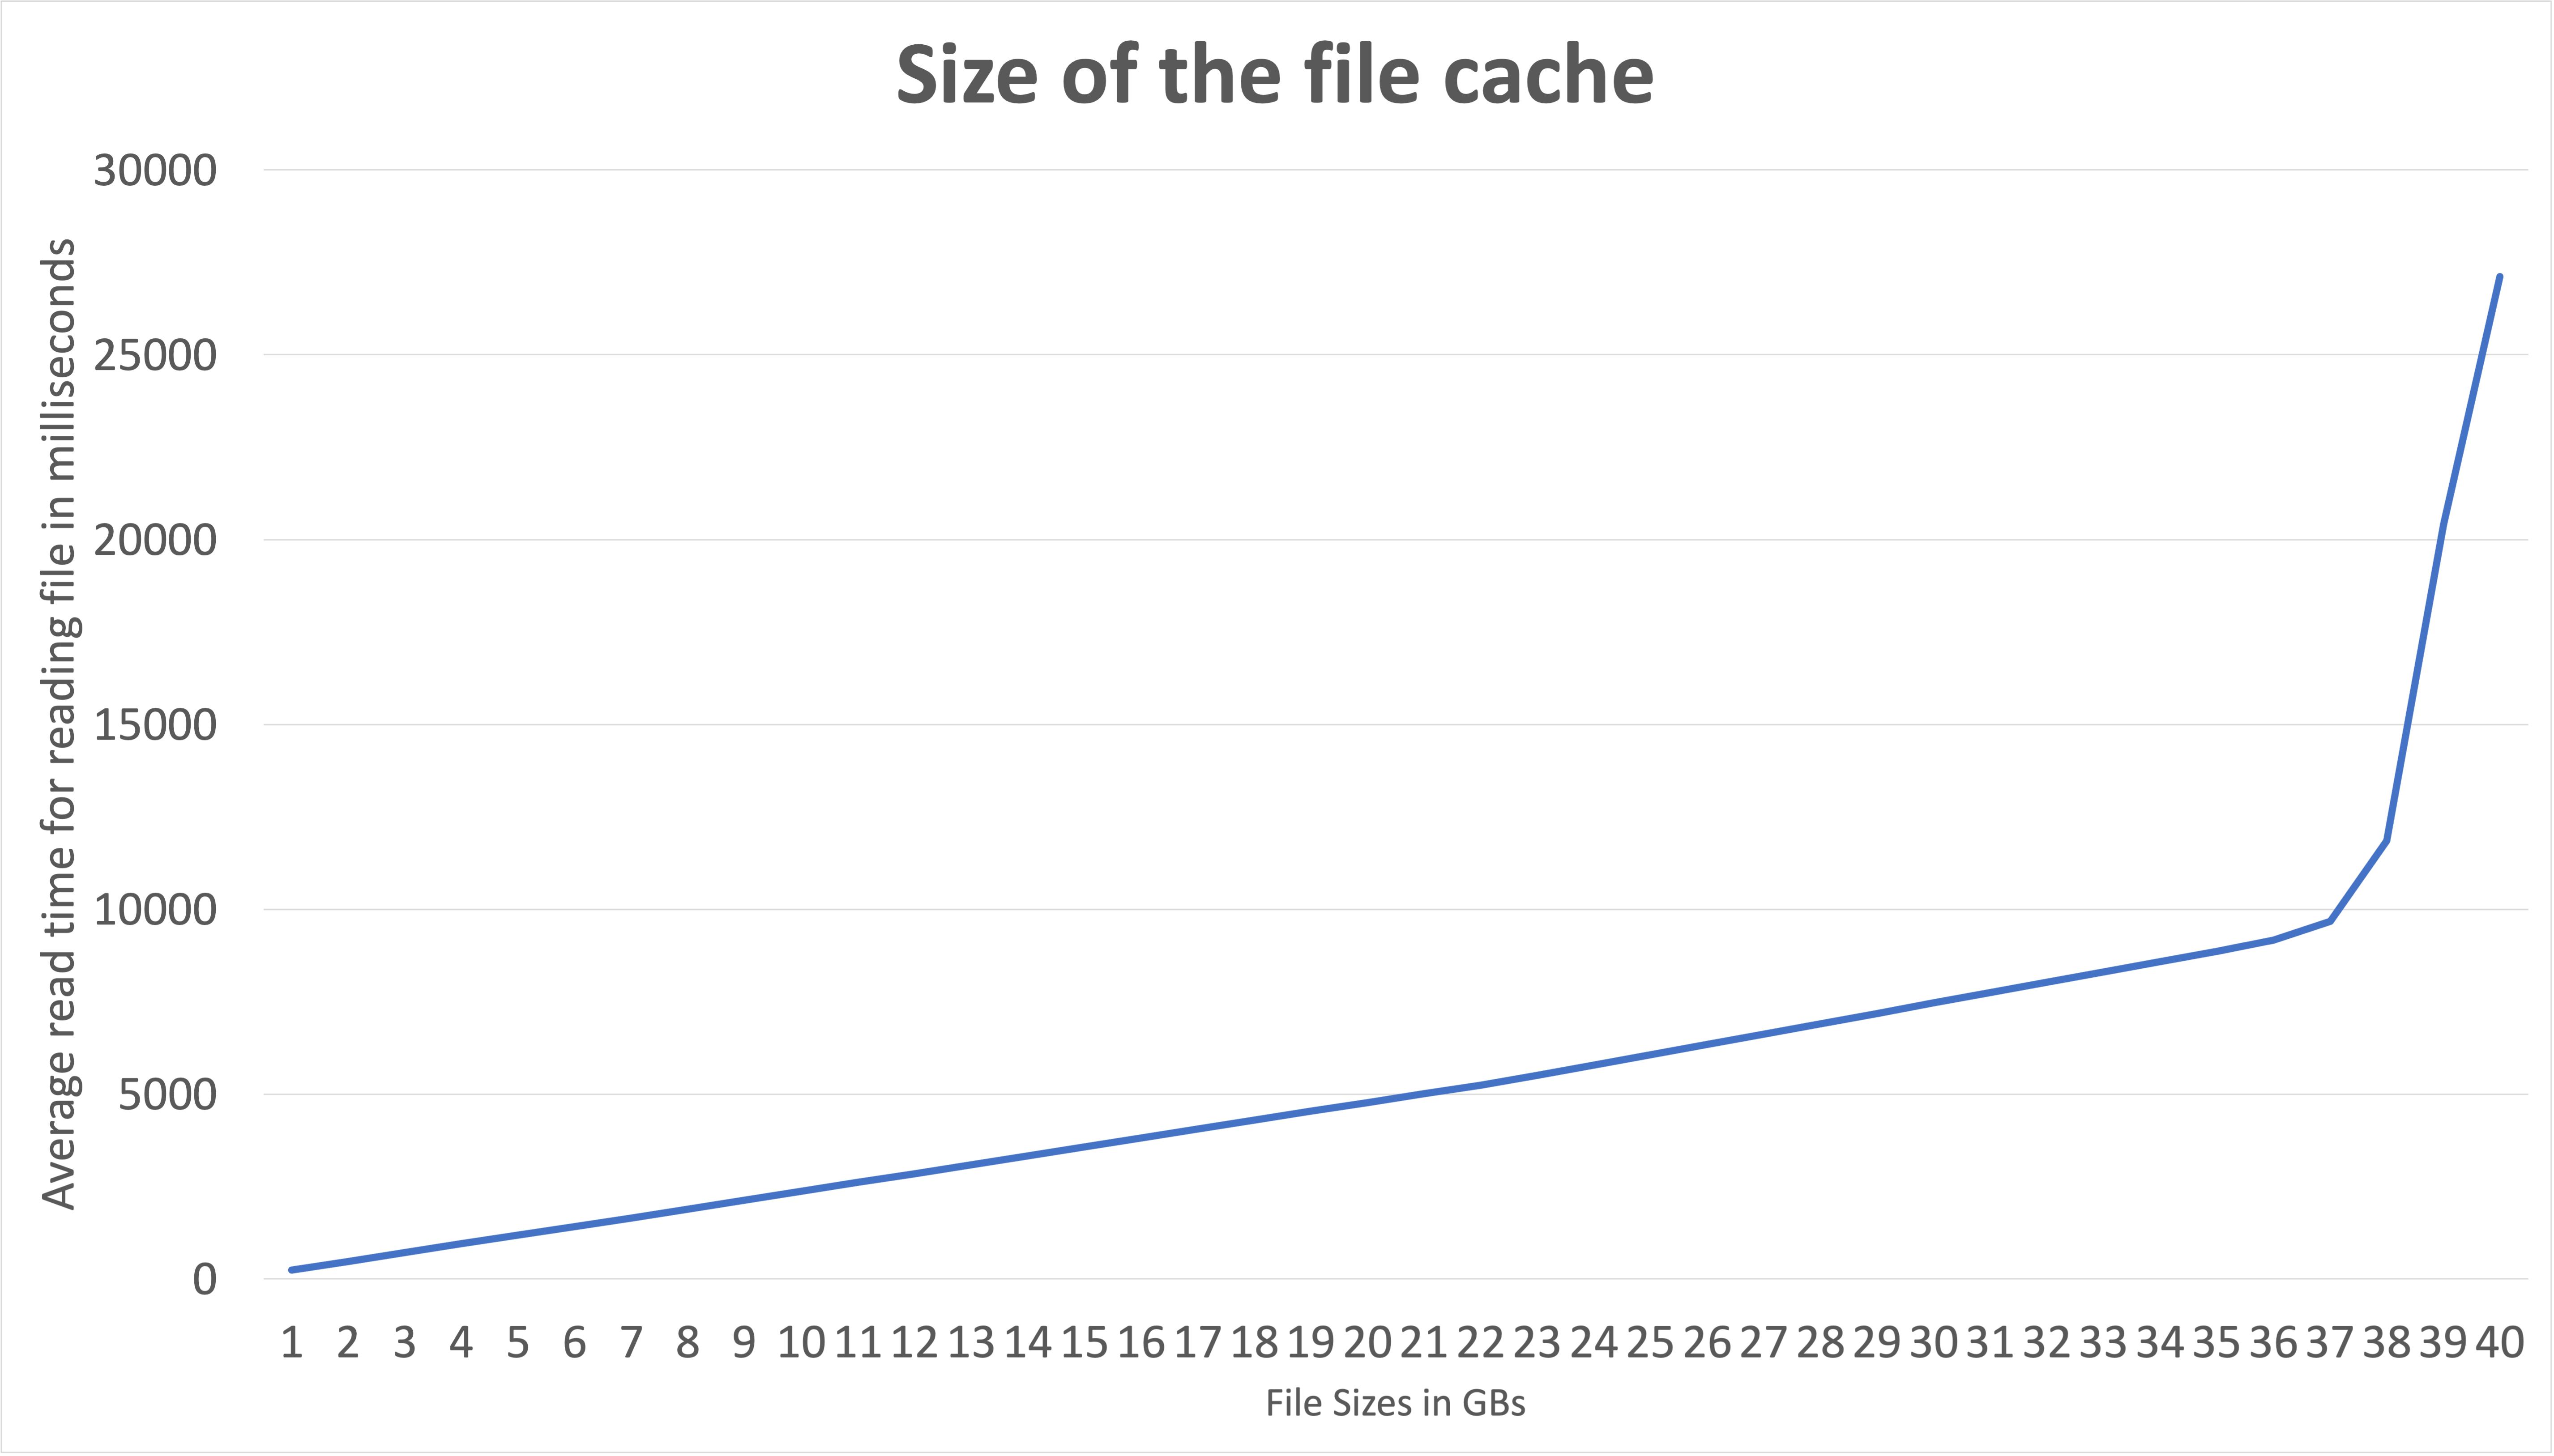
\includegraphics[width=9cm]{size_file_cache.png}

\paragraph{Analysis}

In our graph we can see that there is quite a linear increase in time to read the file from 1GB to around 38GB. Then at around 39GB there is a large increase spike almost doubling the read time. We claim that the file cache size is 38GB because beyond that point there is a huge increase in read time which signifies now requiring a disk read after that file size. Our system uses ZFS for the file system and it uses free RAM as the file cache so we observe that our file cache size grows to be equivalent to be our total available RAM.

\subsubsection{File read time} 

% Report for both sequential and random access as a function of file size. Discuss the sense in which your "sequential" access might not be sequential. Ensure that you are not measuring cached data (e.g., use the raw device interface). Report as a graph with a log/log plot with the x-axis the size of the file and y-axis the average per-block time.

\paragraph{Methodology}

For the file read time, we are asked to compare the difference in time between sequential and random access. Sequential and random access have very distinct characteristics. When sequential access reading is performed, the information is read from the beginning of the file in \emph{sequence} -- one sequential block after another. In contrast, random access reading allows the system read information anywhere in the file. Sequential access has the characteristic of being faster than than random access. Sequential reading was popular back when data was stored on tapes. Random access allows for easier changes to writing. For example, it would be more work to split tape and insert data than it is for random access to rewrite the data on the file.

For our methodology we decided to make a program that generates text files. For each line in the text file, an integer is added. Starting from zero and going to \emph{n}. Within the program the first generated file starts small and increases in size as it progresses. For the sequential method, the generated file is opened and read line by line and each line is added to an array data structure. For random access, the method reads the same file. However, a random number is generated within the range of [0 - \emph{n}]. The program then reads the file and searches for the number. Once the number is found it then goes back to the beginning of the file and looks for the new generated number. Once each number is found, they too are loaded onto an array data structure. This simulates the program reading the file and storing the data somewhere to be used at a later date. The time is takes for sequential and random reading to occur for various file sizes are recorded separately.

This program attempted to simulated sequential access reading as accurately as possible. However, it is possible that this method may not ideally be sequential. This is because it is possible that the file system may pre-allocate some space (extended, JFS) even when the request for little space for it has been make. Once a file has reached a specific size, the file system may need to find another space to store the additional content. If this occurs, the read may not be sequential. Therefore, in order to avoid it, it is useful to pre-allocate the space desired.

\paragraph{Estimate}

We estimate that as the file size increases, it will take exponentially longer for random file read time, when compared to sequential. As previously discussed, it is known that sequential reads are faster when compared to random. Thus, the time will be relatively negligible for the smaller files and will become more significant as the file grows in size.

\paragraph{Results}

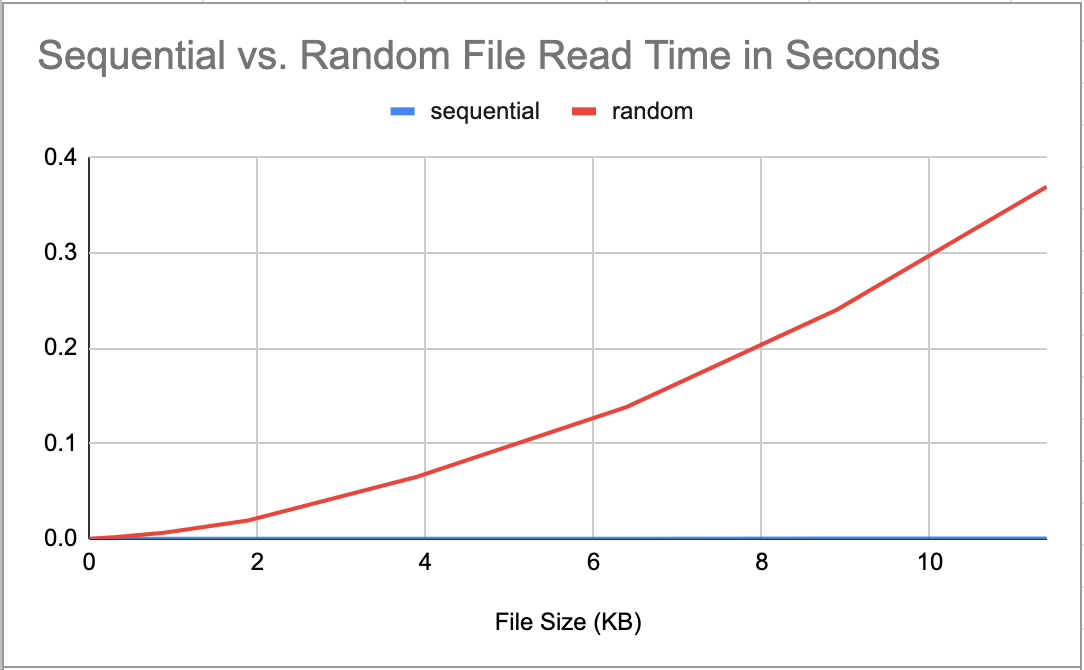
\includegraphics[width=8.5cm]{4.2 Results/Sequential vs. Random File Read Time in Seconds.png}
\hspace{.5cm}
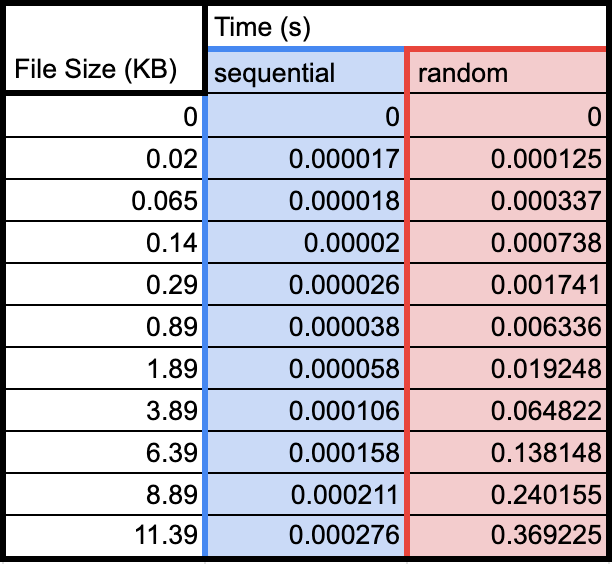
\includegraphics[width=6.5cm]{4.2 Results/Graph Sequential vs. Random File Read Time in Second.png}

\hspace{.25cm}

\includegraphics[width=8.5cm]{4.2 Results/Sequential vs. Random File Read Time in µSeconds.png}
\hspace{.5cm}
\includegraphics[width=6.5cm]{4.2 Results/Graph Sequential vs. Random File Read Time in µSeconds.png}

\hspace{.25cm}

\includegraphics[width=8.5cm]{4.2 Results/Sequential vs. Random File Read Time in log(µSeconds).png}
\hspace{.5cm}
\includegraphics[width=6.5cm]{4.2 Results/Graph Sequential vs. Random File Read Time in log(µSeconds).png}

\paragraph{Analysis}

Based off the results, it appears that our original estimate is correct. As the file size increased, the difference in time between sequential and random reading became more significant. For a small file of 0.020KB, the difference was only 112 µseconds on average. For comparison, for a file the size of 11.4KB, the difference in time is over 350k µseconds on average. Based on the graphs, we can also see that sequential time is much less affected by size. From the smallest file size , 0.020KB, to the largest, 11.4KB, the difference in time was 259 µseconds on average. For comparison, the difference between the same files sizes respectively for random access reading was over 350k µseconds on average. Due to the trends within the graphs, we estimate that this gap will only continue to grow with increased file sizes.

\subsubsection{Remote file read time}

% Repeat the previous experiment for a remote file system. What is the "network penalty" of accessing files over the network? You can either configure your second machine to provide remote file access, or you can perform the experiment on a department machine (e.g., APE lab). On these machines your home directory is mounted over NFS, so accessing a file under your home directory will be a remote file access (although, again, keep in mind file caching effects).

\paragraph{Methodology}

For this section, we are asked to also compare the difference in reading times between sequential access and random access. However, this test involves reading a file over a network. Due to the nature of network, this additional component will add extra time to the entire process known as the \emph{network penalty}

In order to measure the time difference we will roughly be doing the same thing as the last procedure. A text file will be created and read. The random access reading will still be responsible for finding a specific line in the file while the sequential method is able to read the file from start to finish. However, this time both methods will be reading the file over a network. In order to ensure this process executes, we set up an NFS server using the host mentioned from the previous network section. The program running locally, writes and creates files on that server and then they are read by the local program.

\paragraph{Estimate}

We estimate that the remote addition will indeed increase the time significantly for both sequential and random read times. We are curious to see how much of a difference the times are, because this additional time may favor the random access reading times. Thus, it is possible that the sequential reading access's benefit of being superior in speeds locally, will become negligible when measured over a network.

\paragraph{Results}

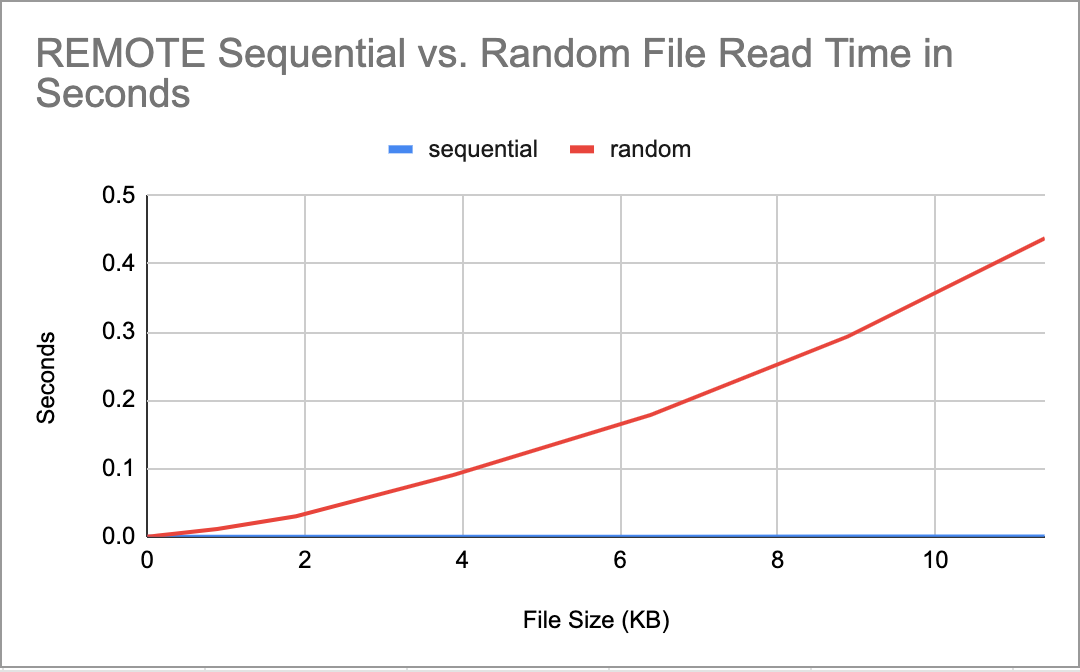
\includegraphics[width=6.5cm]{4.3 Results/my graph seconds.png}
\hspace{.5cm}
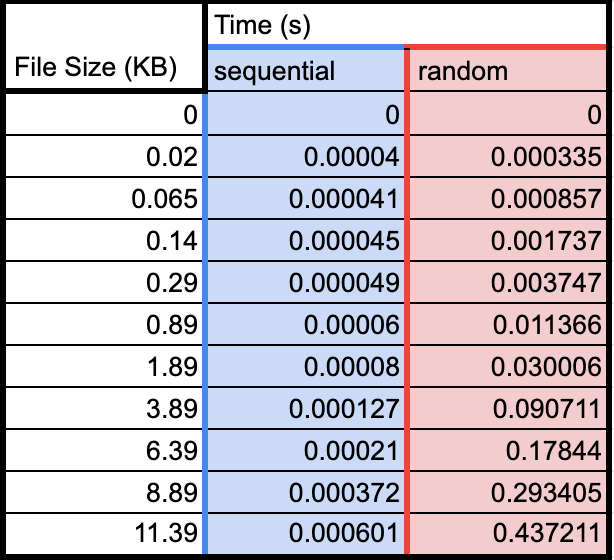
\includegraphics[width=6.5cm]{4.3 Results/table remote seconds.png}

\hspace{.25cm}

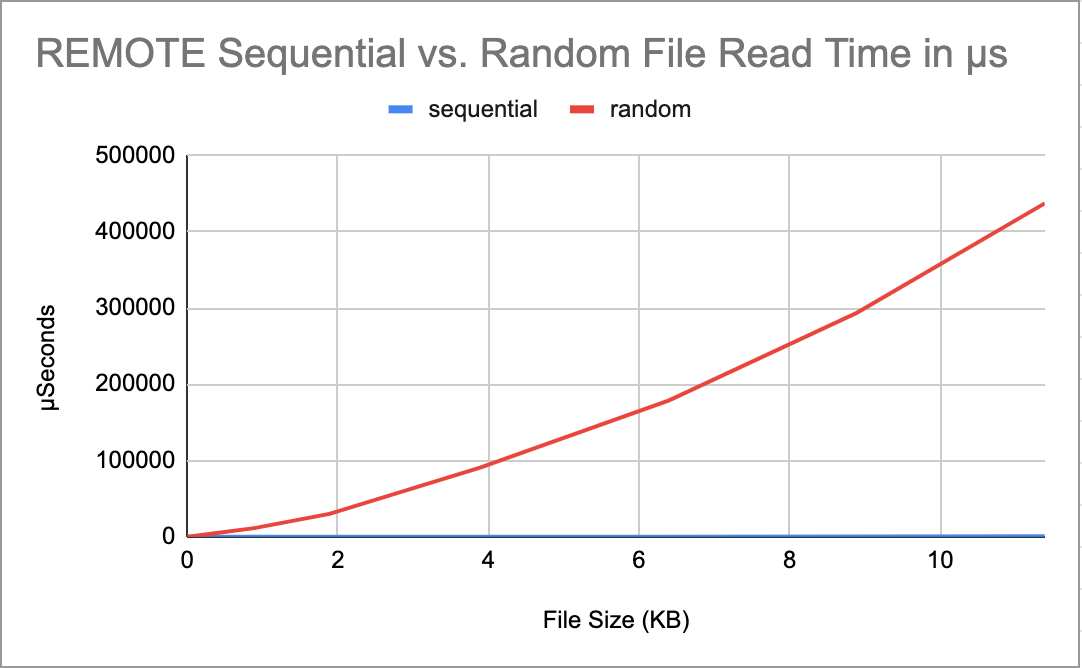
\includegraphics[width=6.5cm]{4.3 Results/my graph microseconds.png}
\hspace{.5cm}
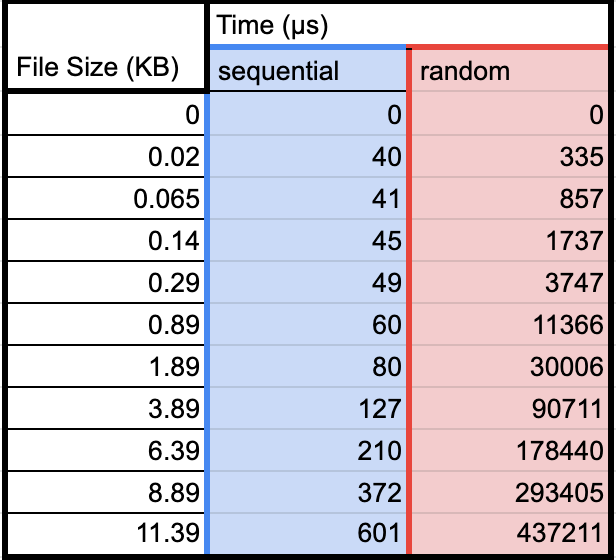
\includegraphics[width=6.5cm]{4.3 Results/table remote microseconds.png}

\hspace{.25cm}

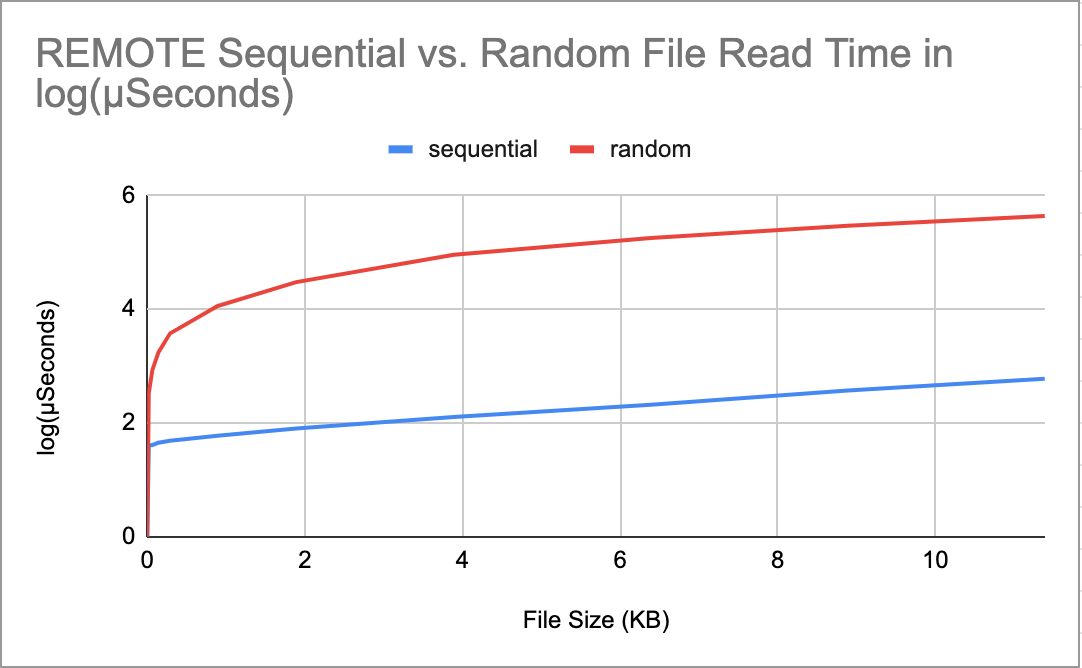
\includegraphics[width=6.5cm]{4.3 Results/my graph log micro.png}
\hspace{.5cm}
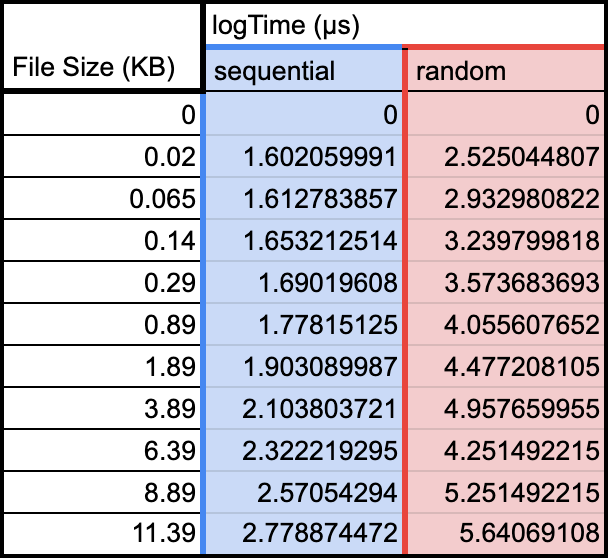
\includegraphics[width=6.5cm]{4.3 Results/table remote log micro.png}

\hspace{.25cm}

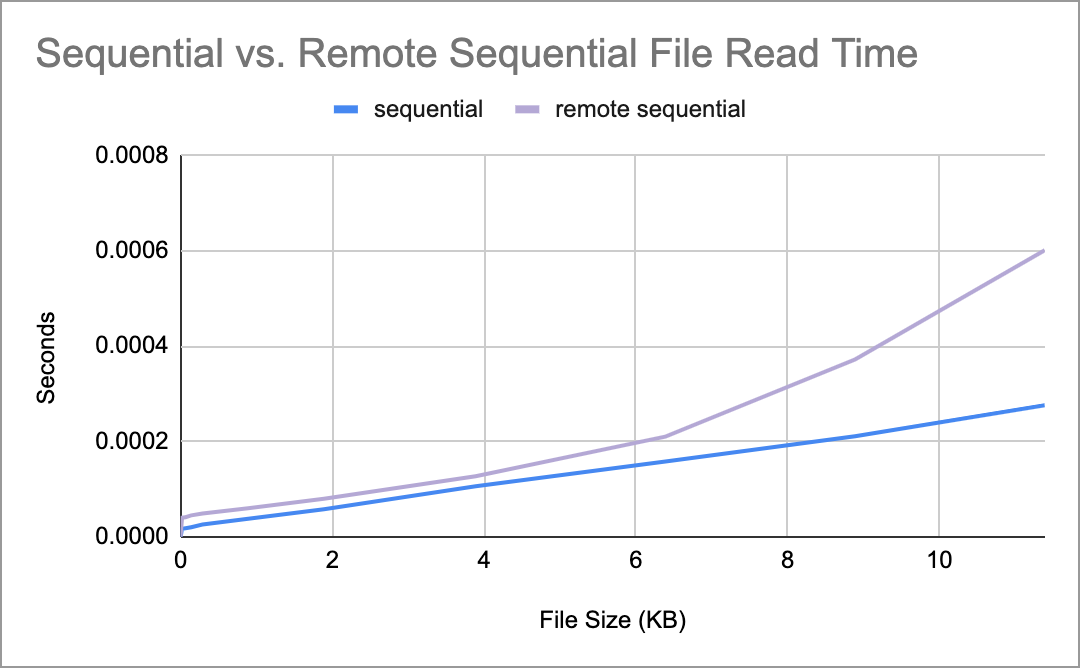
\includegraphics[width=6.5cm]{4.3 Results/s vs rs graph.png}
\hspace{.5cm}
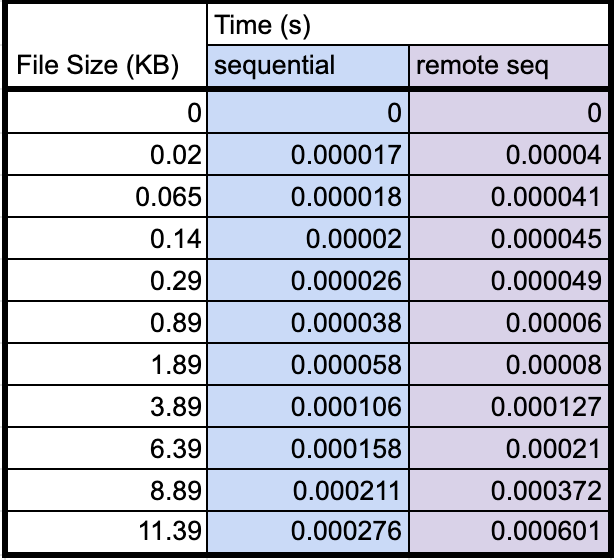
\includegraphics[width=6.5cm]{4.3 Results/table s vs rs.png}

\hspace{.25cm}

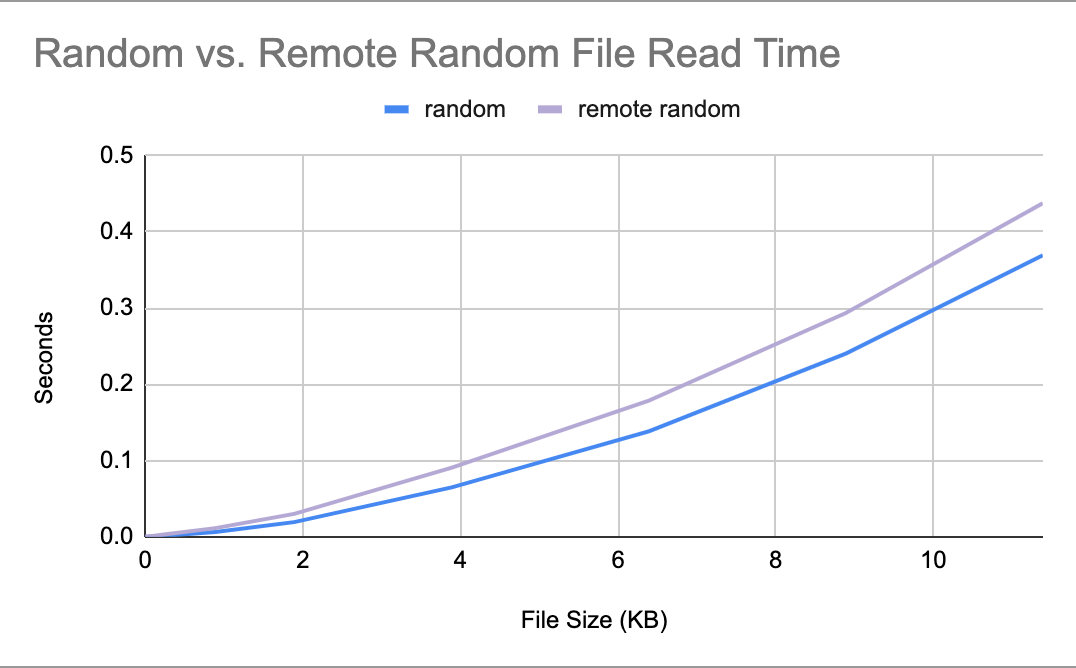
\includegraphics[width=6.5cm]{4.3 Results/r vs rr graph.png}
\hspace{.5cm}
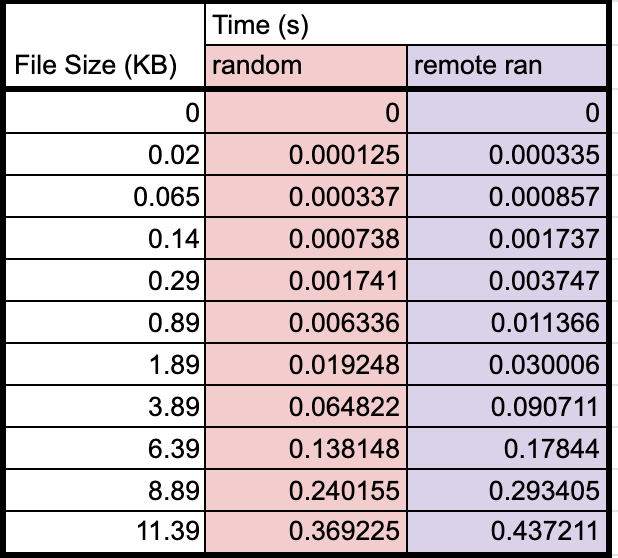
\includegraphics[width=6.5cm]{4.3 Results/table r v rr.png}

\hspace{.25cm}


\paragraph{Analysis}

This test yielded some interesting results. As predicted, accessing the files remotely did indeed increase the time it took for each process to complete regardless of if it was reading through sequential access or random access. When analyzing the graph comparing remote sequence to remote random in µseconds, we can see that sequential access is still clearly much faster than random access. When comparing the smallest and largest files, 0.020KB and 11.4KB respectively, the time difference for sequential access was 561 µseconds on average. For random access on the same files, the time difference for sequential access was over 430K µseconds on average.

The results provide some interesting insights when you compare the original reading times of sequential access and random access processes. Provided above, are two graphs comparing the local and remote times of sequential access and random access respectively. It appears that as the file size increases, the time between local and remote sequential access become increasingly significant. For the comparison of remote and local sequential access, the difference in time for the smallest file is only 13 µseconds. Whereas the difference for the largest file size between local and remote sequential access was 325 µseconds. For the same file sizes, difference in time between local and remote random access for the smallest file was 210 µseconds on average and 67986 µseconds. While this may seems drastic for random access, when assessing the graphs we can see that the local and remote random access lines are much more similar to each other than the local and remote sequential lines. Therefore, due to the remote sequential's line nature to turn exponential, we predict that as the file size increases, sequential access reading time will become more insignificant and eventually negligible.

\subsubsection{Contention}

%Report the average time to read one file system block of data as a function of the number of processes simultaneously performing the same operation on different files on the same disk (and not in the file buffer cache).

\paragraph{Methodology}

For measuring file read contention average time with multiple processes simultaneously we create a C program that opens the file, allocates a block size buffer that we confirmed to be 4096 bytes. We read the file in block size chunks until we have read in 64MB, we time this entire process and note the time it took to read that entire file. So a singular process will do this, to perform this experiment we will create multiple processes that simultaneously run the C program and open different files. We use a bash script that loops through from 1 to 10 which is the number of processes we want to execute at once. The script will create a command that runs the C program on $n$ separate files where $n$ is the current number of processes the experiment is running on. \\
The time recorded is then written out to a file and used in the calculation of our averages over ten trials. With the ZFS system we cannot effectively disable file caching, we try to avoid caching by creating new files for each trial.

\paragraph{Estimate}

As we have more processes running simultaneously we predict that our average time to read a file system block will increase as well. When number of processes increases then we have less effective use of disk and the access time across all processes and different files should be increasing. There can be outliers in our output for page faults to consider and the reading file to use a system call which we have observed overhead for in part 3.1.3. Furthermore since we are having multiple processes run we have context switching overhead potentially as we increase the number of processes and the scheduler will try to give each process a fair distribution of resources; this overhead has been experimented in 3.1.5. Overall, we predict that as the number of simultaneous processes increases we will incur various overheads that cause the access time to increase for all processes.

\paragraph{Results}

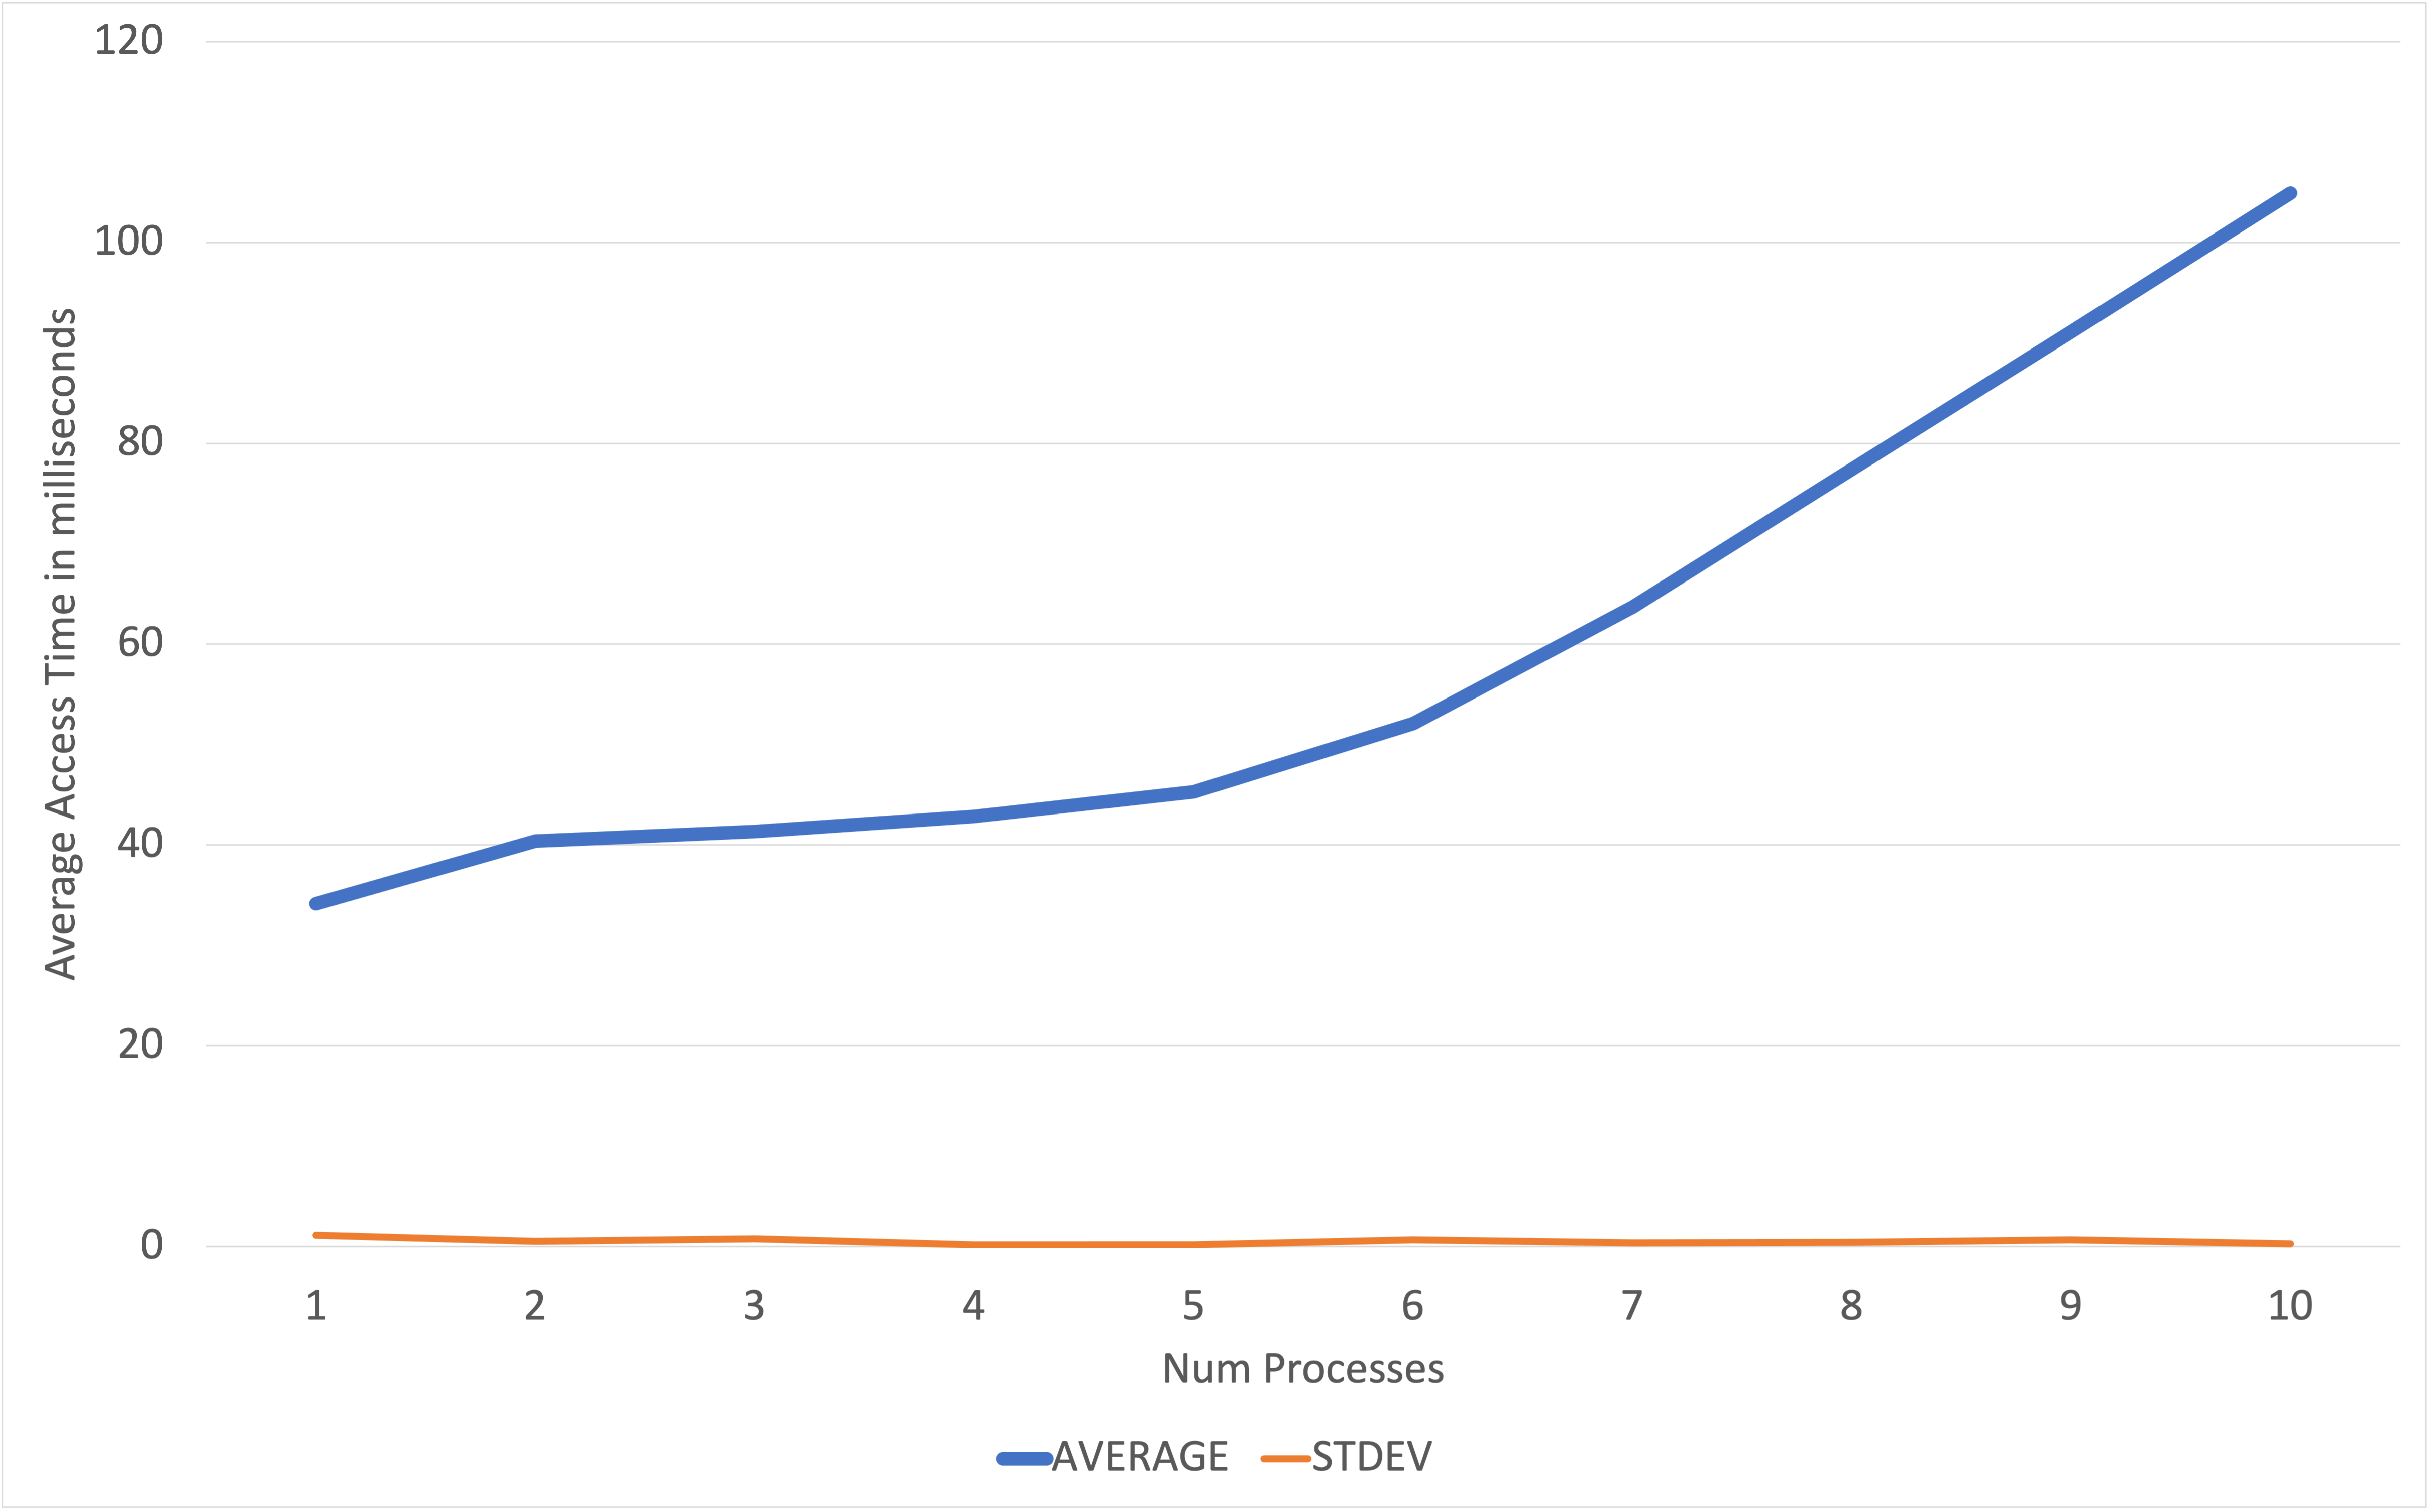
\includegraphics[width=9.5cm]{contention.png}

\paragraph{Analysis}

The results graph shows results that are similar to what we expected in our prediction. When number of processes increase then the average block access time increases somewhat linearly. There is quite little standard deviation showing that these results are acceptable. Keeping everything the same, as we increase the number of simultaneous processes we see performance drawbacks as we have more simultaneous processes. \\
We analyze when there are more processes reading various different files, the current running process may be interrupted and then its data blocks may be flushed out meaning when it continues it has no advantage with prefetching data. Furthermore as more processes are reading from disk they will need to split disk bandwidth. Ultimately the results are acceptable, and in line with our prediction that increasing the amount of parallel processes will also increase the average read time.

%-------------------------------------------------------------------------------
\section*{Availability}
%-------------------------------------------------------------------------------

Code will be on private \href{https://github.com/NeverBehave/cse221-project}{Github Repo} for collaborate purposes, and will be sent on request.

%-------------------------------------------------------------------------------
\bibliographystyle{plain}
\bibliography{references}

%%%%%%%%%%%%%%%%%%%%%%%%%%%%%%%%%%%%%%%%%%%%%%%%%%%%%%%%%%%%%%%%%%%%%%%%%%%%%%%%
\end{document}
%%%%%%%%%%%%%%%%%%%%%%%%%%%%%%%%%%%%%%%%%%%%%%%%%%%%%%%%%%%%%%%%%%%%%%%%%%%%%%%%

%%  LocalWords:  endnotes includegraphics fread ptr nobj noindent
%%  LocalWords:  pdflatex acks
